\chapter{Linux Kernel}
\section{Kernel编译}
\subsection{安装必要的软件包}
\begin{code-block}{bash}
yum install ncurses-devel bison flex elfutils-libelf-devel bc openssl-devel -y
\end{code-block}

\subsection{设置编译选项}
\begin{code-block}{bash}
make menuconfig
\end{code-block}

\subsection{编译内核}
\begin{code-block}{bash}
make
# 如果是在多核服务器上进行编译,可以增加编译参数,提高编译速度
# make -j32 #32表示cpu的核数
\end{code-block}

\subsection{安装内核模块}
\begin{code-block}{bash}
make modules_install
\end{code-block}

安装内核模块的操作,会将编译生成的内核模块复制到/lib/modules/\{kernel-version\}/下。

\subsection{安装内核}
\begin{code-block}{bash}
make install
\end{code-block}

安装内核的过程主要完成了以下的工作:将编译内核时生成的内核镜像bzImage拷贝到/boot目录下,
并将这个镜像命名为vmlinuz-\{kernel-version\}。如果使用x86的cpu,则该镜像位于arch/x86/boot/目录下;
将目录下的System.map拷贝到/boot/目录下,重新命名为System.map-\{kernel-version\},该文件中存放了内核的符号表。
将目录下的.config拷贝到/boot/目录下,重新命名为config-\{kernel-version\}

\subsection{创建initrd.img文件}
\begin{code-block}{bash}
mkinitrd  /boot/initrd.img-{kernel-version} {kernel-version}
\end{code-block}

initrd.img即为初始化的ramdisk文件,它是一个镜像文件。

\subsection{修改grub}
\begin{code-block}{bash}
grub2-mkconfig -o /boot/grub2/grub.cfg
\end{code-block}

修改完成之后,重启服务器,即可发现新编译的内核,如下图\nameref{fig:new-kernel}
\begin{figure}[H]
  \centering
  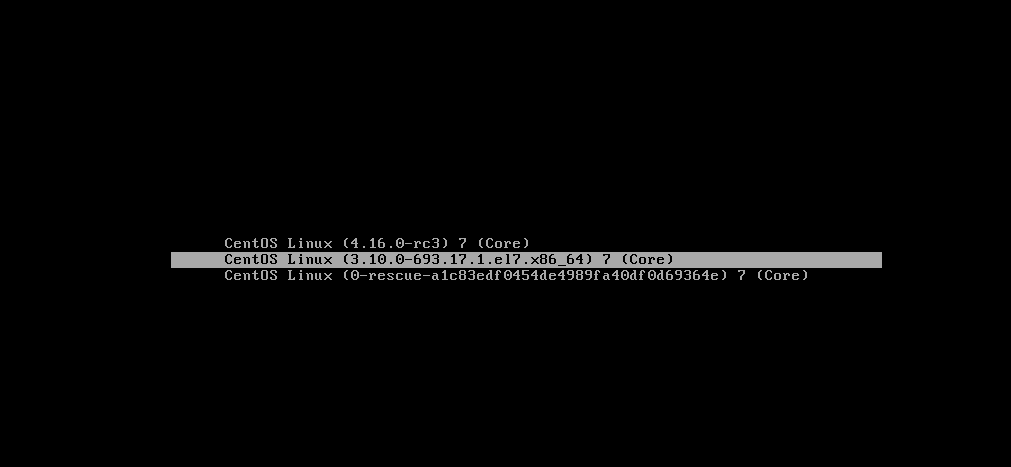
\includegraphics[scale=0.2]{new-kernel.png}
  %\caption{新编译内核 \protect\footnotemark}
  \caption{新编译内核}
  \label{fig:new-kernel}
\end{figure}

\section{编写自己的内核模块}
在编写自己的内核模块的时候,一般需要2个文件:一个c代码文件,包含了自己的内核模块
内在逻辑实现;一个makefile文件,用于编译自己的内核模块。以最简单的hello world为例。
C代码如下:
\begin{code-block}{c}
// hello_kernel.c
#include <linux/init.h>
#include <linux/module.h>
#include <linux/kernel.h>

// 必须,标明模块的许可声明
MODULE_LICENSE("GPL");

// 模块的加载函数,即加载该模块之后,执行的操作
static int hello_init(void)
{
    printk(KERN_ALERT "hello,I am zhangjl\n");
    return 0;
}

// 模块的卸载函数,即该模块卸载之后,应当执行什么操作
static void hello_exit(void)
{
    printk(KERN_ALERT "goodbye,kernel\n");
}

// 注册模块对应的操作
module_init(hello_init);
module_exit(hello_exit);

// 可选,表示该模块的作者和其他信息
MODULE_AUTHOR("zhangjl");
MODULE_DESCRIPTION("This is a simple example!\n");
MODULE_ALIAS("A simplest example");
\end{code-block}

Makefile文件内容如下:
\begin{code-block}{make}
obj-m += hello_kernel.o
#generate the path
CURRENT_PATH:=$(shell pwd)
#the current kernel version number
LINUX_KERNEL:=$(shell uname -r)
#the absolute path
LINUX_KERNEL_PATH:=/usr/src/kernels/$(LINUX_KERNEL)
#complie object
all:
        make -C $(LINUX_KERNEL_PATH) M=$(CURRENT_PATH) modules
#clean
clean:
        make -C $(LINUX_KERNEL_PATH) M=$(CURRENT_PATH) clean
\end{code-block}

然后执行make。执行完毕之后,会在当前目录生成hello\_kernel.ko,这个文件即是我们
所需要的内核模块。执行insmod hello\_kernel.ko,在/var/log/message当中,会发现有hello的输出,执行
rmmod hello\_kernel,在/var/log/message当中,会发现有goodbyd的输出。整个简单的模块
就算完成了。另外,printk函数带缓冲,如果格式化是不添加换行符,则printk所打印的日志并不会
立刻打印出来,有可能会等到模块退出,或者遇到另外一个换行符才会输出。

需要注意这里的license问题。如果license存在问题,或者没有license,会导致编译的内核模块
被加载时,会提示被污染。而合法可用的license如下:
\begin{itemize}
  \item GPL-1.0
  \item ISC
  \item Linux-OpenIB
  \item X11
  \item Apache-2.0
  \item CDDL-1.0
  \item MPL-1.1
  \item GCC-exception-2.0
  \item BSD-2-Clause
  \item Linux-syscall-note
  \item BSD-3-Clause
  \item BSD-3-Clause-Clear
  \item GPL-2.0
  \item LGPL-2.0
  \item LGPL-2.1
  \item MIT
  \item Proprietary
\end{itemize}

其中Proprietary表示私有协议。

\section{导出内核函数}
\begin{code-block}{c}
#include <linux/init.h>
#include <linux/module.h>

#define DRIVER_VERSION  "1.0.0"
#define DRIVER_AUTHOR   "zhangjl luoyan_cn@outlook.com"
#define DRIVER_DESC     "export for example"
#define DRIVER_LICENSE  "Apache-2.0"

int add_int(int a, int b)
{
        return a+b;
}

int sub_int(int a, int b)
{
        return a-b;
}

MODULE_VERSION(DRIVER_VERSION);
MODULE_AUTHOR(DRIVER_AUTHOR);
MODULE_DESCRIPTION(DRIVER_DESC);
MODULE_LICENSE(DRIVER_LICENSE);

EXPORT_SYMBOL(add_int); // 导出函数
EXPORT_SYMBOL(sub_int); // 导出函数
\end{code-block}

该模块进行编译之后,通过insmod加载到内核空间之后,可以通过grep指令进行查询。
\begin{code-block}{bash}
grep add_int /proc/kallsyms
\end{code-block}
一切正常的话,结果大致如下图\nameref{fig:export}所示:
\begin{figure}[H]
  \centering
  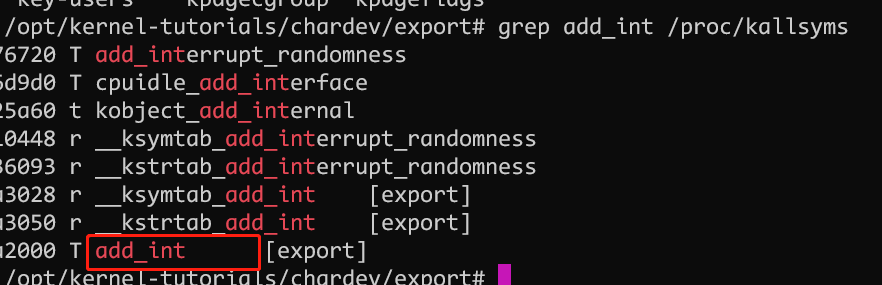
\includegraphics[width=\linewidth]{export.png}
  \caption{内核函数导出}
  \label{fig:export}
\end{figure}

在其他的内核模块当中使用导出的函数,则需要修改相关的定义即可,大致的代码如下:
\begin{code-block}{c}
#include <linux/module.h>
...
extern int add_int(int, int);
extern int sub_int(int, int);
...
static __init int hello_init(void)
{
    int result = 0;
    result = add_int(4, 5);
...
}
\end{code-block}

\section{内核模块参数支持}
\begin{code-block}{c}
#include <linux/module.h>
#include <linux/init.h>

#define DRIVER_VERSION  "1.0.0"
#define DRIVER_AUTHOR   "zhangjl luoyan_cn@outlook.com"
#define DRIVER_DESC     "Params Modules for example"
#define DRIVER_LICENSE  "Apache-2.0"

static char * book_name = "Dive into Linux Kernel";
static int num = 400;

static __init int params_init(void)
{
        printk(KERN_INFO "This is my params modules\n");
        printk(KERN_INFO "Book name is %s\n", book_name);
        printk(KERN_INFO "Book num is %d\n", num);
        return 0;
}

static __exit void params_exit(void)
{
        printk(KERN_INFO "Goodbye, my kernel module\n");
}

module_param(num, int, S_IRUGO); // 表示内核加载时可以接收参数,参数类型为int
module_param(book_name, charp, S_IRUGO); // 表示内核加载的参数为chapr,即char*类型

MODULE_VERSION(DRIVER_VERSION);
MODULE_AUTHOR(DRIVER_AUTHOR);
MODULE_DESCRIPTION(DRIVER_DESC);
MODULE_LICENSE(DRIVER_LICENSE);

module_init(params_init);
module_exit(params_exit);
\end{code-block}

内核模块编译完成之后,可以使用modinfo进行查看,比如modinfo params.ko,其结果大致
如下图\nameref{fig:params}所示:
\begin{figure}[H]
  \centering
  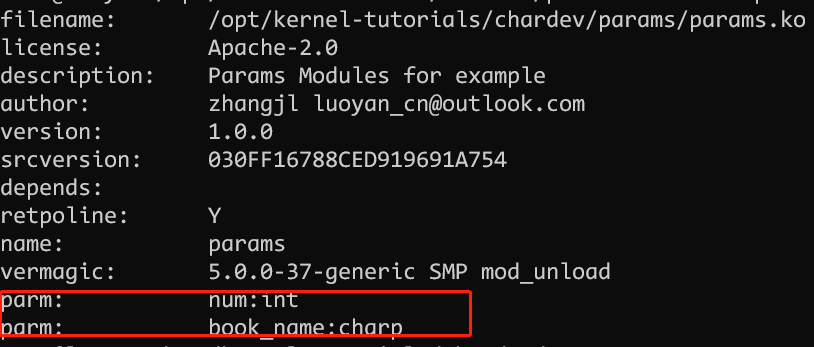
\includegraphics[width=\linewidth]{params.png}
  \caption{内核模块函数参数}
  \label{fig:params}
\end{figure}

使用的时候,可以直接在insmod之后添加参数:
\begin{code-block}{bash}
insmod params.ko book_name=zhangjl num=100
# 传递包含空格的字符串
insmod params.ko book_name='"zhangjl and his family"' num=100
\end{code-block}
内核模块加载之后,查看日志,会有如下图\nameref{fig:params_out}的输出:
\begin{figure}[H]
  \centering
  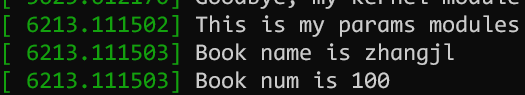
\includegraphics[width=\linewidth]{params_out.png}
  \caption{内核模块函数参数}
  \label{fig:params_out}
\end{figure}

\section{内核模块与版本号}
每一个版本的内核都有自己的版本号描述,而这些版本号描述,会直接影响内核模块的工作。
而内核的版本号是根据git信息自动生成的,具体是通过内核代码当中的scripts/setlocalversion
这个脚本生成的。执行该脚本,其输出如下图\nameref{fig:version}所示:
\begin{figure}[H]
  \centering
  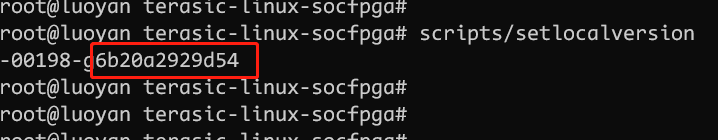
\includegraphics[width=\linewidth]{version.png}
  \caption{获取内核代码版本信息}
  \label{fig:version}
\end{figure}
其中,上述信息的最后部分,刨去开头的g这个字母,剩下的部分,则表示对应的git commit id。
除此之外,内核的版本信息,在进行内核代码编译的时候,也会使用这个脚本进行生成,生成的版本
信息id会保存在内核代码的include/generated/utsrelease.h和include/config/kernel.release文件当中,
在编译内核模块时,如果需要修改这个版本信息,只需要修改include/generated/utsrelease.h当中的
信息即可。

\section{代码判断内核版本号和系统架构}
不同的内核版本,头文件路径可能不同,结构体定义可能不同,函数或者宏定义也可能不同。因此,针对
不同的版本,相应的内核驱动代码通常需要进行适配。而这个适配工作可以直接在代码当中自动完成。如下
代码所示:
\begin{code-block}{c}
#include <linux/version.h>

// 如果内核代码版本小于5.0.0版本
#if LINUX_VERSION_CODE < KERNEL_VERSION(5, 0, 0)
#include <linux/device.h>
#endif

...
#if defined(__arm__)
        printk(KERN_INFO
                "The count of user namespace write is %d\n", count);
#else
        printk(KERN_INFO
                "The count of user namespace write is %ld\n", count);
#endif
\end{code-block}

\section{字符设备驱动开发}
字符设备的注册,需要在init函数当中调用register\_chrdev函数,该函数有几个参数:
\begin{itemize}
    \item \mint{c}|unsigned int major| 表示字符设备的主设备号。
    \item \mint{c}|const char *name|表示字符设备的名称
    \item \mint{c}|const struct file_operations *fops| 表示字符设备的对应操作函数结构体
\end{itemize}

在Linux当中,每个设备都对应了一个设备号,而设备号分为主设备号与次设备号。主设备号
表示某一个具体的驱动,次设备号表示使用该驱动的各个设备。表示设备号的数据结构是dev\_t,
其定义在include/linux/types.h当中,不过实际上,dev\_t就是unsigned int的这么一个无符号的32位
整型数据。而dev\_t的高12位为主设备号,低20位为次设备号,因此,主设备号的取值范围为1-4095(2的12次方)。
而关于设备号的处理,在include/linux/kdev\_t.h当中提供了几个宏定义:

\begin{code-block}{c}
#define MINORBITS     20     // 表示次设备号位数
#define MINORMASK     ((1U << MINORBITS) - 1) // 次设备号掩码
#define MAJOR(dev)    ((unsigned int) ((dev) >> MINORBITS)) // 从dev_t当中获取主设备号
#define MINOR(dev)    ((unsigned int) ((dev) & MINORMASK))  // 从dev_t当中获取次设备号
#define MKDEV(ma,mi)  (((ma) << MINORBITS) | (mi)) // 使用主设备号与次设备号组合成dev_t的设备号
\end{code-block}
在使用的时候,通常无需直接导入kdev\_t.h,只需要使用include/linux/fs.h即可。

默认情况下,使用register\_chrdev会注册字符设备,但是不会创建对应的设备文件(/dev),因此,需要
手动的创建。手动创建字符设备的操作如下:
\begin{code-block}{bash}
mknod /dev/starter c 200 0
\end{code-block}
其中,c表示字符设备,200表示对应设备的主设备号,0表示对应设备的次设备号。

而结构体file\_operations包含了很多的文件操作函数,这些操作函数与用户空间的特定的操作函数
是一一对应的。
\begin{itemize}
    \item open对应open函数(fcntl.h)
    \item release对应close函数(unistd.h)
    \item read对应read函数(unistd.h)
    \item write对应write函数(unistd.h)
\end{itemize}

除了这些常用的函数之外,内核当中的file\_operations包含的函数操作以及相关含义如下:
\begin{itemize}
    \item \mint[linenos=false,breaklines=true,breakanywhere,breaksymbolleft=,breakanywheresymbolpre=,]{c}|loff_t (*llseek) (struct file *, loff_t, int)|llseek方法用作改变文件中的当前读/写位置,
        并且新位置作为(正的)返回值.  loff\_t 参数是一个“long offset”,
        并且就算在32位平台上也至少64位宽. 错误由一个负返回值指示.
        如果这个函数指针是NULL,seek调用会以潜在地无法预知的方式修改file结构中的位置计数器
    \item \mint[linenos=false,breaklines=true,breakanywhere,breaksymbolleft=,breakanywheresymbolpre=,]{c}|unsigned int (*poll) (struct file *, struct poll_table_struct *)|poll方法是3个系统调用的后端:
        poll, epoll, 和 select, 都用作查询对一个或多个文件描述符的读或写是否会阻塞。
        poll方法应当返回一个位掩码指示是否非阻塞的读或写是可能的, 并且, 可能地,
        提供给内核信息用来使调用进程睡眠直到 I/O 变为可能。如果一个驱动的poll方法为NULL,
        设备假定为不阻塞地可读可写。
    \item \mint[linenos=false,breaklines=true,breakanywhere,breaksymbolleft=,breakanywheresymbolpre=,]{c}|int (*ioctl) (struct inode *, struct file *, unsigned int, unsigned long)|ioctl系统调用提供了
        发出设备特定命令的方法(例如格式化软盘的一个磁道, 这不是读也不是写)。
        另外, 几个ioctl命令被内核识别而不必引用fops表。如果设备不提供ioctl方法,
        对于任何未事先定义的请求(-ENOTTY, 设备无这样的ioctl), 系统调用返回一个错误。
    \item \mint[linenos=false,breaklines=true,breakanywhere,breaksymbolleft=,breakanywheresymbolpre=,]{c}|int (*mmap) (struct file *, struct vm_area_struct *)|mmap用来请求将设备内存映射
        到进程的地址空间. 如果这个方法是NULL, mmap系统调用返回-ENODEV。
    \item \mint[linenos=false,breaklines=true,breakanywhere,breaksymbolleft=,breakanywheresymbolpre=,]{c}|int (*flush) (struct file *)|flush操作在进程关闭它的设备文件描述符的拷贝时调用;
        它应当执行(并且等待)设备的任何未完成的操作。这个必须不要和用户查询请求的fsync操作混淆了。
        当前, flush 在很少驱动中使用。
    \item \mint[linenos=false,breaklines=true,breakanywhere,breaksymbolleft=,breakanywheresymbolpre=,]{c}|int (*fsync) (struct file *, struct dentry *, int)|这个方法是fsync系统调用的后端,
        用户调用来刷新任何挂着的数据。如果这个指针是NULL, 系统调用返回-EINVAL。
    \item \mint[linenos=false,breaklines=true,breakanywhere,breaksymbolleft=,breakanywheresymbolpre=,]{c}|int (*fasync) (int, struct file *, int)|这个操作用来通知设备它的FASYNC标志的改变
    \item \mint[linenos=false,breaklines=true,breakanywhere,breaksymbolleft=,breakanywheresymbolpre=,]{c}|int (*lock) (struct file *, int, struct file_lock *)|lock 方法用来实现文件加锁;
        加锁对常规文件是必不可少的特性, 但是设备驱动几乎从不实现它。
\end{itemize}

一个简单的字符驱动的框架大致如下:
\begin{code-block}{c}
#include <linux/fs.h>
#include <linux/init.h>
#include <linux/kernel.h>
#include <linux/module.h>

#define MARJOR 200
#define DEV_NAME "starter"

static int open_starter_chrdev(struct inode *inodep, struct file *filep)
{
        printk(KERN_INFO "Open the starter char dev \n");
        return 0;
}

static int release_starter_chrdev(struct inode *inodep, struct file *filp)
{
        printk(KERN_INFO "Close the starter char dev \n");
        return 0;
}

static ssize_t read_starter_chrdev(struct file *filp,
                char __user * buffer, size_t count, loff_t *ppos)
{
        printk(KERN_INFO "Read the starter char dev \n");
        return 0;
}

static ssize_t write_starter_chrdev(struct file *filp,
                const char __user *buffer, size_t count, loff_t *ppos)
{
        printk(KERN_INFO "Write the starter char dev \n");
        return 0;
}

static struct file_operations starter_fops = {
        .owner = THIS_MODULE,
        .open = open_starter_chrdev,
        .release = release_starter_chrdev,
        .read = read_starter_chrdev,
        .write = write_starter_chrdev,
};

static int __init starter_init(void)
{
        int result = 0;
        result = register_chrdev(MARJOR, DEV_NAME, &starter_fops);
        if (0 > result) {
                printk(KERN_ERR
                        "Failed to register the starter char device\n");
                return result;
        }
        printk(KERN_INFO
                "This is a starter module for char dev init function\n");
        return 0;
}

static void __exit starter_exit(void)
{
        printk(KERN_INFO
                "This is a starter module for char dev exit function\n");
        unregister_chrdev(MARJOR, DEV_NAME);
}

MODULE_LICENSE("Apache-2.0");
MODULE_AUTHOR("zhangjl");
MODULE_DESCRIPTION("This is a simple example!\n");
MODULE_ALIAS("A simplest example");

module_init(starter_init);
module_exit(starter_exit);
\end{code-block}

\section{驱动的读写操作函数}
在Linux驱动的操作函数当中,read/write是比较常用的。其中内核驱动的read/write函数接口定义如下:
\begin{code-block}{c}
ssize_t (*read) (struct file *, char __user *, size_t, loff_t *);
ssize_t (*write) (struct file *, const char __user *, size_t, loff_t *);
\end{code-block}
read函数,通常的功能在于,从内核空间读取数据到用户空间;而write则反过来,从用户
空间写数据到内核空间。常见的read/write函数的实现大致如下:
\begin{code-block}{c}
// linux/uaccess.h copy_to_user, copy_from_user

/*
*** buffer:用户空间缓冲区,在内核空间当中,无法直接访问,不能进行printk
*** count:用户空间读取的缓冲区大小
*** ppos:偏移地址
*/
static ssize_t read_starter_chrdev(struct file *filp,
        char __user * user_buffer, size_t count, loff_t *ppos)
{
        int ret = 0;
        struct chrdev * char_device = (struct chrdev*)filp->private_data;
#if defined(__arm__)
        printk(KERN_INFO "The count of user"
                        " namespace requested is %d\n", count);
#else
        printk(KERN_INFO "The count of user"
                        " namespace requested is %ld\n", count);
#endif
        // 偏移量超过了最大的长度
        if (*ppos > BUFFER_LEN) {
                return count ? -ENXIO : 0;
        }
        // 偏移量超过了剩余长度
        if (count > (BUFFER_LEN - *ppos)) {
                count = BUFFER_LEN - *ppos;
        }
        // *ppos表示偏移量的地址
        if ((ret = copy_to_user(
                user_buffer, (void *)(char_device->buffer + *ppos), count))) {
                printk(KERN_ERR "Faichrdev to read data from kernel\n");
                return -EFAULT;
        }
        *ppos += count; // 必须进行该操作,否则会出现不可预知的问题
#if defined(__arm__)
        printk(KERN_INFO "The count of copy_to_user is %d\n", count);
#else
        printk(KERN_INFO "The count of copy_to_user is %ld\n", count);
#endif
        return count;
}

/*
*** buffer:用户空间缓冲区,在内核空间当中,无法直接访问,不能进行printk
*** count:用户空间写入的缓冲区大小
*** ppos:偏移地址
*/
static ssize_t write_starter_chrdev(struct file *filp,
        const char __user * user_buffer, size_t count, loff_t *ppos)
{
        int ret = 0;
        struct chrdev * char_device = (struct chrdev*)filp->private_data;
#if defined(__arm__)
        printk(KERN_INFO
                "The count of user namespace write is %d\n", count);
#else
        printk(KERN_INFO
                "The count of user namespace write is %ld\n", count);
#endif
        if (count >= BUFFER_LEN) {
                return count ? -ENXIO : 0;
        }
        if (count > (BUFFER_LEN - *ppos)) {
                count = BUFFER_LEN - *ppos;
        }

        if ((ret = copy_from_user(char_device->buffer+*ppos,
                                user_buffer, count))) {
                printk(KERN_ERR "Faichrdev write to char device\n");
                return -EFAULT;
        }

        *ppos += count; // 必须进行该操作,否则会出现不可预知的问题
        printk(KERN_INFO "Write to the chrdev"
                " char dev with content %s\n",                                                                                                                               char_device->buffer);
        return count;
}
\end{code-block}

需要注意,用户空间缓冲区,在内核空间是不能直接进行操作的,必须通过copy\_to\_user和copy\_from\_user
进行,否则会导致操作系统直接卡住。除此之外,需要特别注意,read/write函数的返回值,如果一切运行正常,
返回值应当为操作的数量(即count),不能随意返回0,否则,在使用cat/echo等命令对字符设备文件进行操作时,
会导致操作系统卡住(使用代码进行读写的方式运行正常)。

另外,在上述的代码当中,首次出现了一个-EFAULT的标记,这个表示Linux的内核错误代码。在Linux内核代码当中,
存在一系列关于各种错误的定义,这些错误的定义全部都在include/uapi/asm-generic/errno-base.h当中,而典型的
Linux错误代码包括如下的内容:
\begin{code-block}{c}
#define EPERM   1  /* Operation not permitted */
#define ENOENT  2  /* No such file or directory */
#define ESRCH   3  /* No such process */
#define EINTR   4  /* Interrupted system call */
#define EIO     5  /* I/O error */
#define ENXIO   6  /* No such device or address */
#define E2BIG   7  /* Argument list too long */
#define ENOEXEC 8  /* Exec format error */
#define EBADF   9  /* Bad file number */
#define ECHILD  10 /* No child processes */
#define EAGAIN  11 /* Try again */
#define ENOMEM  12 /* Out of memory */
#define EACCES  13 /* Permission denied */
#define EFAULT  14 /* Bad address */
#define ENOTBLK 15 /* Block device required */
#define EBUSY   16 /* Device or resource busy */
#define EEXIST  17 /* File exists */
#define EXDEV   18 /* Cross-device link */
#define ENODEV  19 /* No such device */
#define ENOTDIR 20 /* Not a directory */
#define EISDIR  21 /* Is a directory */
#define EINVAL  22 /* Invalid argument */
#define ENFILE  23 /* File table overflow */
#define EMFILE  24 /* Too many open files */
#define ENOTTY  25 /* Not a typewriter */
#define ETXTBSY 26 /* Text file busy */
#define EFBIG   27 /* File too large */
#define ENOSPC  28 /* No space left on device */
#define ESPIPE  29 /* Illegal seek */
#define EROFS   30 /* Read-only file system */
#define EMLINK  31 /* Too many links */
#define EPIPE   32 /* Broken pipe */
#define EDOM    33 /* Math argument out of domain of func */
#define ERANGE  34 /* Math result not representable */
\end{code-block}

\section{设备号的动态分配}
在上述操作当中,我们必须手动的指定设备号,并且手动的创建设备节点,才可以对其进行
操作和访问。但是,Linux提供了一套设备驱动的框架,支持进行自动的设备号分配,以及
设备节点的自动创建。

自动申请设备号采用下列函数进行操作:
\begin{code-block}{c}
/**
* dev 表示设备号,
* baseminor 表示基础的次设备号,即从多少开始进行次设备号的分配
* count 表示申请多少个
* name 表示设备的名称
*/
int alloc_chrdev_region(dev_t *dev, unsigned baseminor,
    unsigned count, const char *name);

// 其使用方式大致如下:

ret = alloc_chrdev_region(&devid, 0, MAX_COUNT, "device_name");
// 获取主设备号
major = MAJOR(devid);
minor = MINOR(devid);
\end{code-block}

如果指定了主设备号,但是自动分配次设备号,可以采用下面的类似代码进行:
\begin{code-block}{c}
int register_chrdev_region(dev_t from, unsigned count, const char *name);

// 其使用方式大致如下:
devid = MKDEV(major,0);
ret = register_chrdev_region(devid, MAX_COUNT, "device_name");
\end{code-block}

相应的,卸载设备则应该使用对应的函数:
\begin{code-block}{c}
void unregister_chrdev_region(dev_t from, unsigned count)
\end{code-block}

\section{字符设备的注册}
虽然可以使用register\_chrdev进行字符设备的注册,但是,很多时候,我们通常采用的是
更为现代的方式和函数。新的字符设备的注册,需要使用到一个特殊的结构体——cdev:
\begin{code-block}{c}
// linux/cdev.h
struct cdev {
        struct kobject kobj;
        struct module *owner;
        const struct file_operations *ops;
        struct list_head list;
        dev_t dev;
        unsigned int count;
} __randomize_layout;
\end{code-block}
然后,使用cdev\_init函数对字符设备进行注册,随后使用cdev\_add函数将字符设备添加到
Linux操作系统当中。基本的操作大致如下,定义一个设备结构体,包含上述的cdev结构体,并且
包含主设备号,次设备号以及本身的设备号dev\_id:
\begin{code-block}{c}
struct devframework {
        dev_t dev_id;
        unsigned int major;
        unsigned int minor;
        struct cdev frame_cdev;
};

static struct devframework item;

static struct file_operations devframework_fops = {
        .owner = THIS_MODULE,
        .open = open_devframework_chrdev,
        .release = release_devframework_chrdev,
        .read = read_devframework_chrdev,
        .write = write_devframework_chrdev,
};

static int __init devframework_init(void)
{
        int result = 0;
        // 从Linux系统当中申请设备号
        result = alloc_chrdev_region(&item.dev_id, 0, 1, DEV_NAME);
        if (result) {
                printk(KERN_ERR
                        "Faild devframework to register"
                        " the devframework char device\n");
                return -EFAULT;
        }

        // 获取主设备号与次设备号
        item.major = MAJOR(item.dev_id);
        item.minor = MINOR(item.dev_id);
        item.frame_cdev.owner = THIS_MODULE;
        // 初始化设备,进行注册,包含了设备的文件操作函数
        cdev_init(&item.frame_cdev, &devframework_fops);
        // 添加设备到操作系统当中
        if ((result = cdev_add(&item.frame_cdev, item.dev_id, 1))){
                printk(KERN_ERR "Faild to add devframework"
                                " into Linux system\n");
                return -ENODEV;
        }
        printk(KERN_INFO
                "This is a devframework module"
                " for char dev init function,"
                " and major is %d, minor is %d\n",
                item.major, item.minor);
        return result;
}

static void __exit devframework_exit(void)
{
        printk(KERN_INFO
                "This is a devframework module"
                " for char dev exit function\n");
        // 从操作系统当中卸载设备
        cdev_del(&item.frame_cdev);
        // 回收注册的设备号
        unregister_chrdev_region(item.dev_id, 1);
}
\end{code-block}

\section{自动创建设备文件}
之前创建设备采用的是mknod的方式(即devfs),属于静态创建的方式。从Linux2.6之后,
采用了udev的方式,进行设备的创建。而udev的方式,直接可以管理/dev下的设备文件,并且支持
热插拔方式,因此,得到极大的发展。自动创建设备文件,通常采用函数device\_create完成。
将上述的内容的综合到一起,得到一个比较完整的字符驱动(以框架的形式运行),其代码大致如下:
\begin{code-block}{c}
#include <linux/version.h>
#include <linux/cdev.h>
#include <linux/fs.h>
#include <linux/init.h>
#include <linux/kernel.h>
#include <linux/module.h>
#include <linux/uaccess.h>

#if LINUX_VERSION_CODE < KERNEL_VERSION(5, 0, 0)
#include <linux/device.h>
#endif

#define DEV_NAME "chrdev"
#define BUFFER_LEN 1024

// 定义设备结构体
// 定义设备结构体
struct chrdev {
        dev_t          dev_id;  // 设备id
        unsigned int   major;   // 主设备号
        unsigned int   minor;   // 次设备号
        struct device  *device; // device结构体指针,用于创建对应的设备文件
        struct class   *class;  // class结构体指针,用于创建对应的设备类型
        struct cdev    *cdev;   // cdev结构体指针,用于注册字符设备
        char           buffer[BUFFER_LEN];
};

static struct chrdev char_device;
// 默认的主设备号为0
static unsigned int major = 0;
// 添加内核模块的参数支持,支持通过参数传递major的数值
module_param(major, uint, S_IRUGO)

static int open_chrdev(struct inode *inodep, struct file *filp)
{
        // 设置文件的私有变量,后续在驱动的其他操作当中,可以直接
        // 使用filp指针,而无需操作全局的char_device变量
        filp->private_data = &char_device;
        printk(KERN_INFO "Open the char dev named chrdev\n");
        return 0;
}

static int release_chrdev(struct inode *inodep, struct file *filp)
{
        // 从文件的私有变量当中提取设备结构体
        struct chrdev *char_device = (struct chrdev*)filp->private_data;
        printk(KERN_INFO "Close the chrdev char dev \n");
        return 0;
}

static ssize_t read_chrdev(struct file *filp,
        char __user *user_buffer, size_t count, loff_t *ppos)
{
        int ret = 0;
        struct chrdev *char_device = (struct chrdev*)filp->private_data;
#if defined(__arm__)
        printk(KERN_INFO "The count of user"
                " namespace requested is %d\n", count);
#else
        printk(KERN_INFO "The count of user"
                " namespace requested is %ld\n", count);
#endif
        if (*ppos > BUFFER_LEN) {
                return count ? -ENXIO : 0;
        }
        if (count > (BUFFER_LEN - *ppos)) {
                count = BUFFER_LEN - *ppos;
        }
        if ((ret = copy_to_user(user_buffer,
                (void *)(char_device->buffer), count))) {
                printk(KERN_ERR "Faichrdev to read data from kernel\n");
                return -EFAULT;
        }
        *ppos += count;
#if defined(__arm__)
        printk(KERN_INFO "The count of copy_to_user is %d\n", count);
#else
        printk(KERN_INFO "The count of copy_to_user is %ld\n", count);
#endif
        return count;
}

static ssize_t write_chrdev(struct file *filp,
        const char __user *user_buffer, size_t count, loff_t *ppos)
{
        int ret = 0;
        struct chrdev *char_device = (struct chrdev*)filp->private_data;
#if defined(__arm__)
        printk(KERN_INFO
                "The count of user namespace write is %d\n", count);
#else
        printk(KERN_INFO
                "The count of user namespace write is %ld\n", count);
#endif
        if (count >= BUFFER_LEN) {
                return count ? -ENXIO : 0;
        }

        if ((ret = copy_from_user(
                char_device->buffer+*ppos, user_buffer, count))) {
                printk(KERN_ERR "Faichrdev write to char device\n");
                return -EFAULT;
        }

        *ppos += count;
        printk(KERN_INFO "Write to the chrdev"
                " char dev with content %s\n", char_device->buffer);
        return count;
}

static struct file_operations chrdev_fops = {
        .owner   = THIS_MODULE,
        .open    = open_chrdev,
        .release = release_chrdev,
        .read    = read_chrdev,
        .write   = write_chrdev,
};

static int __init chrdev_init(void)
{
        int result = 0;
        if (major > 0) {
                // 根据insmod xxx.ko major=yyy的参数,得到major
                // 然后生成字符设备的设备号
                char_device.dev_id = MKDEV(major, 0);
                // 注册设备的设备号到操作系统
                result = register_chrdev_region(
                        char_device.dev_id, 1, DEV_NAME);
        } else {
                // 申请设备号,0表示次设备号的起始编号,1表示设备的数量
                result = alloc_chrdev_region(
                        &char_device.dev_id, 0, 1, DEV_NAME);
        }
        if (result) {
                printk(KERN_ERR
                        "Faild chrdev to register"
                        " the chrdev char device\n");
                result = -EFAULT;
                goto dev_id_fail;
        }

        char_device.cdev = cdev_alloc();
        if (!char_device.cdev) {
                printk(KERN_ERR "Faild to alloc cdev struct \n");
                result = -EFAULT;
                goto alloc_cdev_fail;
        }

        // 获取主设备号
        char_device.major = MAJOR(char_device.dev_id);
        // 获取次设备号
        char_device.minor = MINOR(char_device.dev_id);
        char_device.cdev->owner = THIS_MODULE;

        // 初始化字符设备,包含字符设备的操作函数
        cdev_init(char_device.cdev, &chrdev_fops);

        // 添加字符设备到操作系统,1表示添加的数量
        if ((result = cdev_add(char_device.cdev, char_device.dev_id, 1))) {
                printk(KERN_ERR "Faild to add chrdev"
                                " into Linux system\n");
                result = -EFAULT;
                goto dev_add_fail;
        }

        // 创建字符设备类型
        char_device.class = class_create(THIS_MODULE, DEV_NAME);
        if(IS_ERR(char_device.class)){
                result = PTR_ERR(char_device.class);
                goto dev_class_fail;
        }

        // 创建字符设备文件,即/dev/下的文件,device_create的4个参数
        // 第一个表示设备类型
        // 第二个表示设备的父设备
        // 第三个表示设备号
        // 第四个表示设备数据
        // 第五个为可变参数,即可以是多个,表示设备的名称
        char_device.device = device_create(char_device.class, NULL,
                char_device.dev_id, NULL, DEV_NAME);
        if (IS_ERR(char_device.device)) {
                result = PTR_ERR(char_device.device);
                goto dev_device_fail;
        }

        memset(char_device.buffer, 0, BUFFER_LEN);

        printk(KERN_INFO "This is a chrdev module"
                " for char dev init function,"
                " and major is %d, minor is %d\n",
                char_device.major, char_device.minor);
        return result;

dev_device_fail:
        class_destroy(char_device.class);
dev_class_fail:
        cdev_del(char_device.cdev);
dev_add_fail:
alloc_cdev_fail:
        unregister_chrdev_region(char_device.dev_id, 1);
dev_id_fail:
        return result;
}

static void __exit chrdev_exit(void)
{
        printk(KERN_INFO
                "This is a chrdev module"
                " for char dev exit function\n");
        // 销毁设备文件
        device_destroy(char_device.class, char_device.dev_id);
        // 销毁设备类型
        class_destroy(char_device.class);
        // 从系统当中删除字符设备
        cdev_del(char_device.cdev);
        // 回收申请到的设备号
        unregister_chrdev_region(char_device.dev_id, 1);
}

module_init(chrdev_init);
module_exit(chrdev_exit);

MODULE_LICENSE("GPL"); // 必须为GPL的license
MODULE_AUTHOR("zhangjl");
\end{code-block}

需要注意的是,一旦使用了上述的这种方式,则内核模块的license必须为GPL,原因是
device\_destroy和class\_destroy都属于GPL的导出函数,与其他的协议不兼容。如果
强制使用其他的协议,则会出现类似下列的错误:
\begin{code-block}{bash}
FATAL: modpost: GPL-incompatible module private.ko uses GPL-only symbol 'device_destroy'
scripts/Makefile.modpost:93: recipe for target '__modpost' failed
make[2]: *** [__modpost] Error 1
\end{code-block}
利用上述的框架,除了在/dev下生成对应的设备文件之外,在/sys/class下也会生成对应的
文件。

如果将上述代码再次进行改写,全部使用指针的形式,则需要在内核当中使用kmalloc/kzalloc/kfree等函数,
用于在内核空间当中申请对应的内存空间,具体的代码如下:
\begin{code-block}{c}
#include <linux/version.h>
#include <linux/cdev.h>
#include <linux/fs.h>
#include <linux/init.h>
#include <linux/kernel.h>
#include <linux/module.h>
#include <linux/slab.h>
#include <linux/uaccess.h>

#if LINUX_VERSION_CODE < KERNEL_VERSION(5, 0, 0)
#include <linux/device.h>
#endif

#define DEV_NAME "chrdev"
#define BUFFER_LEN 1024

struct chrdev {
        dev_t         dev_id;
        unsigned int  major;
        unsigned int  minor;
        struct device *device;
        struct class  *class;
        struct cdev   *cdev;
        char          buffer[BUFFER_LEN];
};

// 定义设备结构体指针,而不再是结构体
static struct chrdev *dev;
static unsigned int major = 0;
module_param(major, uint, S_IRUGO);

static int open_chrdev(struct inode *inodep, struct file *filp)
{
        filp->private_data = dev;
        printk(KERN_INFO "Open the char dev named chrdev\n");
        return 0;
}

static int release_chrdev(struct inode *inodep, struct file *filp)
{
        struct chrdev *dev = (struct chrdev*)filp->private_data;
        printk(KERN_INFO "Close the char dev \n");
        return 0;
}

static ssize_t read_chrdev(struct file *filp,
        char __user * user_buffer, size_t count, loff_t *ppos)
{
        int ret = 0;
        struct chrdev *dev = (struct chrdev*)filp->private_data;
#if defined(__arm__)
        printk(KERN_INFO "The count of user"
                " namespace requested is %d\n", count);
#else
        printk(KERN_INFO "The count of user"
                " namespace requested is %ld\n", count);
#endif
        if (*ppos > BUFFER_LEN) {
                return count ? -ENXIO : 0;
        }

        if (count > (BUFFER_LEN - *ppos)) {
                count = BUFFER_LEN - *ppos;
        }

        if ((ret = copy_to_user(
                user_buffer, (void *)(dev->buffer+*ppos), count))) {
                printk(KERN_ERR "Failed to read data from kernel\n");
                return -EFAULT;
        }

        *ppos += count;
        return count;
}

static ssize_t write_chrdev(struct file *filp,
        const char __user *user_buffer, size_t count, loff_t *ppos)
{
        int ret = 0;
        struct chrdev *dev = (struct chrdev*)filp->private_data;
#if defined(__arm__)
        printk(KERN_INFO "The count of user namespace write is %d\n", count);
#else
        printk(KERN_INFO "The count of user namespace write is %ld, %lld\n",
                count, *ppos);
#endif
        if (count >= BUFFER_LEN) {
                return count ? -ENXIO : 0;
        }
        // 如果需要每次都覆盖内存当中的内容,需要进行原始内容清空
        // memset(dev->buffer, 0, BUFFER_LEN);
        if ((ret = copy_from_user(dev->buffer+*ppos, user_buffer, count))) {
                printk(KERN_ERR "Faichrdev write to char device\n");
                return -EFAULT;
        }
        *ppos += count;
        printk(KERN_INFO "Write to the char dev with content %s\n",
                dev->buffer);
        return count;
}

static struct file_operations chrdev_fops = {
        .owner   = THIS_MODULE,
        .open    = open_chrdev,
        .release = release_chrdev,
        .read    = read_chrdev,
        .write   = write_chrdev,
};

static int __init chrdev_init(void)
{
        int result = 0;
        // 申请内核空间的内存使用kmalloc和kzalloc,但是通常使用kzalloc
        // 原因在于kzalloc申请内存之后,自动将对应的内存区域进行清空置零
        // 而kmalloc并不会。另外,kzalloc在底层默认就是调用kmalloc函数进行的
        // 操作
        // dev = kmalloc(sizeof(struct chrdev), GFP_KERNEL);
        dev = kzalloc(sizeof(struct chrdev), GFP_KERNEL);
        if (!dev) {
                result = -ENOMEM;
                goto alloc_kernel_fail;
        }
        if (major > 0) {
                dev->dev_id = MKDEV(major, 0);
                result = register_chrdev_region(dev->dev_id, 1, DEV_NAME);
        } else {
                result = alloc_chrdev_region(&(dev->dev_id), 0, 1, DEV_NAME);
        }
        if (result) {
                printk(KERN_ERR "Faild to register the char device\n");
                result = -EFAULT;
                goto dev_id_fail;
        }

        dev->major = MAJOR(dev->dev_id);
        dev->minor = MINOR(dev->dev_id);

        // 申请一个cdev指针
        dev->cdev = cdev_alloc();
        if (!dev->cdev) {
                printk(KERN_ERR "Faild to alloc cdev struct \n");
                result = -EFAULT;
                goto alloc_cdev_fail;
        }

        dev->cdev->owner = THIS_MODULE;

        // 初始化cdev结构体指针
        cdev_init(dev->cdev, &chrdev_fops);

        if ((result = cdev_add(dev->cdev, dev->dev_id, 1))) {
                printk(KERN_ERR "Faild to add chrdev into Linux system\n");
                result = -EFAULT;
                goto dev_add_fail;
        }

        dev->class = class_create(THIS_MODULE, DEV_NAME);
        if (IS_ERR(dev->class)) {
                result = PTR_ERR(dev->class);
                goto dev_class_fail;
        }

        dev->device = device_create(dev->class, NULL,
                dev->dev_id, NULL, DEV_NAME);
        if (IS_ERR(dev->device)) {
                result = PTR_ERR(dev->device);
                goto dev_device_fail;
        }

        memset(dev->buffer, 0, BUFFER_LEN);

        printk(KERN_INFO "This is a chrdev module"
                " for char dev init function,"
                " and major is %d, minor is %d\n",
                dev->major, dev->minor);
        return result;

dev_device_fail:
        class_destroy(dev->class);
dev_class_fail:
        cdev_del(dev->cdev);
dev_add_fail:
alloc_cdev_fail:
        unregister_chrdev_region(dev->dev_id, 1);
dev_id_fail:
        kfree(dev);
alloc_kernel_fail:
        return result;
}

static void __exit chrdev_exit(void)
{
        printk(KERN_INFO "This is a chrdev module"
                " for char dev exit function\n");
        device_destroy(dev->class, dev->dev_id);
        class_destroy(dev->class);
        cdev_del(dev->cdev);
        unregister_chrdev_region(dev->dev_id, 1);
        // 释放申请的设备结构体指针内存
        kfree(dev);
}

module_init(chrdev_init);
module_exit(chrdev_exit);

MODULE_LICENSE("GPL");
MODULE_AUTHOR("zhangjl");
\end{code-block}

\section{内核的并发与同步}
内核当中也会涉及到并发与同步。最简单的并发控制,便是使用原子操作,限制设备的
并发访问。对上述代码进行改动,就变成了一个只允许同一时间只能有一个访问请求的
驱动,代码的改动如下:
\begin{code-block}{c}
...
static unsigned int major;
// 定义设备同一时间只有一个可用
static atomic_t awcloud_available = ATOMIC_INIT(1);
module_param(major, uint, 0444);
...

static int open_awcloud_mem(struct inode *inodep, struct file *filp)
{
        // 设备已经被打开
        if (!atomic_dec_and_test(&awcloud_available)) {
                atomic_inc(&awcloud_available);
                // 设备正忙
                return -EBUSY;
        }
        filp->private_data = dev;
        return 0;
}

static int release_awcloud_mem(struct inode *inodep, struct file *filp)
{
        // 释放设备
        atomic_inc(&awcloud_available);
        return 0;
}
...
\end{code-block}

但是,同时只允许一个进程访问的设备驱动毕竟是少数,
因此内核当中的并发,通常采用自旋锁以及信号量进行。
自旋锁的主要特点如下:
\begin{itemize}
  \item 忙等待,无调度开销
  \item 禁止进程抢占
  \item 锁定期间不能休眠
\end{itemize}
即访问互斥的临界资源,如果无法拿到对应资源的锁,则自己进行自旋,直到拿到锁为止。
自旋锁的空间也是原子空间,不能执行任何可能引起睡眠的操作。自旋锁不能被任何一个线程
打断,但是可以被中断打断。所以,自旋锁存在一个变体,即spin\_lock\_irqsave,可以保证被
中断打断。单核的情况下,自旋锁退化为禁止内核调度或者抢占。
自旋锁的使用大致如下:
\begin{code-block}{c}
spinlock_t lock;
spin_lock_init(&lock);
spin_lock(&lock);   // 获取自旋锁,保护临界区
...                 // 临界区
spin_unlock(&lock); // 解锁
\end{code-block}
通常,自旋锁用在一段可以在很短的时间内做完的操作当中;如果对应的操作可能存在
休眠,以及需要很长的时间进行操作,则只能使用信号量以及互斥量。

而信号量(互斥量)的特点则如下:
\begin{itemize}
  \item 拿不到需要的资源就进行进程切换,存在调度的开销
  \item 锁定期间可以休眠,但是不用于中断的上下文
\end{itemize}
信号量的使用大致如下:
\begin{code-block}{c}
DECLARE_MUTEX(sem);// 定义信号量
down(&sem); // 获取信号量,保护临界区
... // 临界区
up(&sem); // 释放信号量
\end{code-block}

互斥量的使用大致如下:
\begin{code-block}{c}
// mutex_init(); 动态申请互斥量
static DEFINE_MUTEX(my_mutex); // 静态定义互斥量,通常是全局范围
mutex_lock(&my_mutex);  // 获取互斥量,保护临界区
... // 临界区
mutex_unlock(&my_mutex);// 释放互斥量
\end{code-block}

而内核的同步,即要求某件事情必须先完成,其他事情才可以继续,则通常采用completion和等待队列进行。
Completion的主要作用就是用于同步。其基本的使用如下:
\begin{code-block}{c}
struct completion done;

static int xxx_txrx()
{
        init_completion(&done);
        ...
        wait_for_completion(&done); // 对应进程进入休眠状态,等待事情完成
        ...
}

static irqreturn_t xxx_irq(int irq, void *dev)
{
        ...
        complete(&done);            // 任务完成,唤醒wait_for_completion的进程
        return IRQ_HANDLED;
}
\end{code-block}

等待队列,代表了一些休眠进程的集合。在实际的使用当中,信号量/互斥量以及completion
都需要使用等待队列进行完成。其基本的用法如下:
\begin{code-block}{c}
wait_queue_head_t xxx_wait;

void xxx(...)
{
        // wait和current为内核当中已经存在的2个宏定义
        // 定义等待队列
        DECLARE_WAITQUEUE(wait, current);
        // 添加到等待队列中,唤醒等待队列,就可以唤醒当前的进程
        add_wait_queue(&xxx_wait, &wait);

        do {
                avail = device_writeble(...);
                if (0>avail) {
                        // 改变进程状态,进程进入可打断的休眠态
                        __set_current_state(TASK_INTERRUPTIBLE);
                }
                if (0>avail) {
                        // 非阻塞
                        if(file->f_flags & O_NONBLOCK) {
                            ...
                        }
                        // 调度其他进程执行
                        schedule();
                        // 信号唤醒
                        if (signal_pending(current)) {
                            ...
                        }
                }
        } while(avail<0);
        device_write(...);

        // 从等待队列当中移除
        remove_wait_queue(&xxx_wait, &wait);
        // 设置进程状态为运行
        __set_current_state(TASK_RUNNING);
}
\end{code-block}

\section{内核的延时与定时器以及中断}
内核的延时主要有2种:忙等待和休眠等待。
所谓的忙等待,就是空转,常用的函数包括ndelay,udelay,mdelay等,这些函数会
直接消耗cpu,并且不会将cpu调度给其他的进程,最好不要随意使用只有等待时间很短,
或者对应的任务不能休眠的情况下,才能使用忙等待。其他情况下,通常都是使用休眠
等待,即会将cpu调度给其他进程使用,包括msleep,msleep\_interupptible,ssleep,
sleep\_on\_timeout,interruptible\_sleep\_on\_timeout等。

而为了精确的定义时间,以及定时任务,内核当中包含了一个定时器,其大致的定义如下:
\begin{code-block}{c}
struct timer_list {
        // 定时器列表
        struct list_head entry;
        // 定时器到期时间
        unsigned long expires;
        // 定时器的处理函数
        void (*function)(unsigned long);
        // 定时器处理函数的参数
        unsigned long data;
        struct timer_base_s *base;
};
\end{code-block}
当定时器到期之后,function函数将被执行。一个简单的定时器使用范例如下:
\begin{code-block}{c}
void xxx_func(...)
{
        struct xxx_dev *dev = (struct xxx_dev *)filp->private_data;
        // 初始化定时器
        init_timer(&dev->xxx_timer);
        dev->xxx_timer.function = &xxx_do_timer;

        // 设备结构体指针作为定时器处理函数的参数
        dev->xxx_timer.data = (unsigned long)dev;
        dev->xxx_timer.expires = jiffies + delay;
        //  添加/注册定时器
        add_timer(&dev->xxx_timer);
}

static void xxx_do_timer(unsigned long arg)
{
        // 将指针地址转换为设备指针
        struct xxx_device *dev = (struct xxx_dev *)(arg);
        ...
        // 调度定时器再次执行
        dev->xxx_timer.expires = jiffies + delay;
        add_timer(&dev->xxx_timer);
}
\end{code-block}

在内核当中,中断包含了2部分:中断的上半部以及中断的下半部(底半部)。上半部
是硬件处理机制,而底半部,则是软件的处理,因此通常称之为软中断。

软中断可以采用Tasklet进行操作,其基本的操作如下:
\begin{code-block}{c}
// 定义tasklet与底半部函数,并进行关联
void xxx_do_tasklet(unsigned long);
DECLARE_TASKLET(xxx_tasklet, xxx_do_tasklet, 0);

// 中断处理底半部
void xxx_do_tasklet(unsigned long)
{
        ...
}

// 中断处理顶半部
irqreturn_t xxx_interupt(int irq, void *dev_id, struct pt_regs *regs)
{
        ...
        tasklet_schedule(&xxx_tasklet);
        ...
}
\end{code-block}
当处理不可能出现休眠状态的中断,或者优先级非常高的中断时,可以考虑采用Tasklet;
而如果是处理可能出现休眠状态的中断,则应该考虑使用工作队列(workqueue);而针对
input类型的中断时(比如触摸屏),则应当考虑使用threaded\_irq。

\section{Linux的进程遍历}
一个进程是由进程控制块(PCB),代码段和数据段组成的;并且,OS通常是通过PCB来感知
一个进程的存在。其实PCB就是操作系统对每个进程的代码描述。linux内核中使用task\_struct
结构来描述一个PCB(具体可以在linux/kernel/sched.c查看源码);多个进程则常常使用双链表
等来进行组织。比如可运行状态的进程组成可运行队列,等待状态的进程组成等待队列等。

list\_head为linux内核当中常用的数据结构,用于构造双链表,关于list\_head的具体用法,可以
参见c部分的宏定义高级使用部分。而task\_struct的定义类似于如下的代码:
\begin{code-block}{c}
struct task_struct {
        struct thread_info    thread_info;
        struct list_head      tasks;
};
\end{code-block}

由于该结构体当中存在list\_head的变量,因此,我们可以利用该变量来访问整个task\_strut,
进而获取我们需要的信息。完整代码如下:
\begin{code-block}{c}
#include <linux/init.h>
#include <linux/module.h>
#include <linux/kernel.h>
#include <linux/sched.h>
#include <linux/sem.h>
#include <linux/list.h>

MODULE_LICENSE("GPL");
static int hello_init(void)
{
        printk(KERN_ALERT "hello,I am zhangjl\n");
        return 0;
}

static int traverse_init(void)
{
       struct task_struct *pos;
       struct list_head *current_head;
       int count=0;
       printk("Traversal module is working..\n");
       current_head=&(current->tasks);
       list_for_each_entry(pos,current_head,tasks)
       {
              count++;
              printk("[process %d]: %s\'s pid is %d\n",count,pos->comm,pos->pid);
       }
       printk(KERN_ALERT"The number of process is:%d\n",count);
       return 0;
}

static void hello_exit(void)
{
    printk(KERN_ALERT "goodbye,kernel\n");
    traverse_init();
}

module_init(hello_init);
module_exit(hello_exit);
MODULE_AUTHOR("zhangjl");
MODULE_DESCRIPTION("This is a simple example!\n");
MODULE_ALIAS("A simplest example");

\end{code-block}

其中,current是一个宏,即为系统内正在运行的进程。编译该文件,然后加载该模块,在
系统日志当中,即可发现对应的输出。

\section{内核的IO模型}

在之前的内核代码当中,基本没有考虑任何的并发和并行的情况,因此,如果是针对
一个 设备同时进行操作,就会导致内核出现崩溃。而常用的解决方式,就是进行加锁。
在内核当中,主要有4种I/O模型,可以实现对设备的访问控制:
\begin{itemize}
  \item 阻塞I/O:最常用,最简单
  \item 非阻塞I/O:可以防止进程阻塞在I/O操作当中
  \item I/O多路复用:允许同时对多个I/O进行控制,通常需要实现poll函数
  \item 信号驱动I/O:异步通信模型
\end{itemize}

\subsection{阻塞/非阻塞式I/O}
常用的阻塞式IO通常采用信号量或者互斥量进行,通过对资源的加锁,解决了并发访问
资源的问题。信号量的加锁方式大致如下:
\begin{code-block}{c}
#include <linux/version.h>
#include <linux/cdev.h>
#include <linux/fs.h>
#include <linux/init.h>
#include <linux/kernel.h>
#include <linux/module.h>
#include <linux/slab.h>
#include <linux/uaccess.h>

#if LINUX_VERSION_CODE < KERNEL_VERSION(5, 0, 0)
#include <linux/device.h>
#endif

#define DEV_NAME "awcloud"
#define BUFFER_LEN 4096
#define MEM_CLEAR 0x1

struct awcloud_sem {
        dev_t             dev_id;
        unsigned int      major;
        unsigned int      minor;
        unsigned int      used_len;
        struct device     *device;
        struct class      *class;
        struct cdev       *cdev;
        char              buffer[BUFFER_LEN];
        // 定义一个信号量
        struct semaphore  sem;
};

static struct awcloud_sem *dev;
static unsigned int major;
module_param(major, uint, 0444);

static int open_awcloud_sem(struct inode *inodep, struct file *filp)
{
        filp->private_data = dev;
        return 0;
}

static int release_awcloud_sem(struct inode *inodep, struct file *filp)
{
        return 0;
}

static ssize_t read_awcloud_sem(struct file *filp,
        char __user *user_buffer, size_t count, loff_t *ppos)
{
        int ret = 0;
        struct awcloud_sem *dev = (struct awcloud_sem *)filp->private_data;

        if (*ppos >= BUFFER_LEN) {
                return count ? -ENXIO:0;
        }

        if (count > (BUFFER_LEN - *ppos)) {
                count = BUFFER_LEN - *ppos;
        }

        // 获取信号量,如果失败,则表示有进程已经在访问了,当前不允许访问
        if (down_interruptible(&dev->sem)) {
                return -ERESTARTSYS;
        }

        // 临界区资源
        if (copy_to_user(user_buffer, (void *)(dev->buffer + *ppos), count)) {
                return -EFAULT;
        }

        *ppos += count;
        ret = count;

        // 释放信号量
        up(&dev->sem);

        return ret;
}

static ssize_t write_awcloud_sem(struct file *filp,
        const char __user *user_buffer, size_t count, loff_t *ppos)
{
        int ret = 0;
        struct awcloud_sem *dev = (struct awcloud_sem *)filp->private_data;

        if (*ppos >= BUFFER_LEN) {
                return count ? -ENXIO:0;
        }

        if (count > BUFFER_LEN - *ppos) {
                count = BUFFER_LEN - *ppos;
        }

        pr_info(
#if defined(__arm__)
                "Calling the write function with count %d, and ppos %lld\n",
#else
                "Calling the write function with count %ld, and ppos %lld\n",
#endif
                count, *ppos);

        if (down_interruptible(&dev->sem)) {
                return -ERESTARTSYS;
        }

        if (copy_from_user(dev->buffer + *ppos, user_buffer, count)) {
                ret = -EFAULT;
                return ret;
        }

        *ppos += count;
        if (*ppos > dev->used_len) {
                dev->used_len = *ppos;
        }
        ret = count;

        up(&dev->sem);
        pr_info(
#if defined(__arm__)
                "Release the semaphore of write for count %d\n",
#else
                "Release the semaphore of write for count %ld\n",
#endif
                count);

        return ret;
}

#if LINUX_VERSION_CODE < KERNEL_VERSION(2, 6, 36)
int ioctl_awcloud_sem(struct inode *inodep,
        struct file *filp, unsigned int cmd, unsigned long arg)
{
#else
static long ioctl_awcloud_sem(struct file *filp,
        unsigned int cmd, unsigned long arg)
{
        //struct inode *inodep = file_inode(filp);
#endif
        struct awcloud_sem *dev = (struct awcloud_sem *)filp->private_data;

        switch (cmd) {
        case MEM_CLEAR:
                if (down_interruptible(&dev->sem)) {
                        return -ERESTARTSYS;
                }

                memset(dev->buffer, 0, BUFFER_LEN);
                dev->used_len = 0;

                up(&dev->sem);

                pr_info("Set Kernel Buffer to Zero\n");
                break;
        default:
                return -EINVAL;
        }
        return 0;
}

static loff_t llseek_awcloud_sem(struct file *filp,
        loff_t offset, int whence)
{
        loff_t ret = 0;
        struct awcloud_sem *dev = (struct awcloud_sem *)filp->private_data;

        pr_info(
                "Calling the llseek function of this device,"
                "and offset is %lld , whence is %d\n", offset, whence);
        switch (whence) {
        case SEEK_SET:
                if (offset < 0) {
                        ret = -EINVAL;
                        break;
                }
                if ((unsigned int)offset > BUFFER_LEN) {
                        ret = -EINVAL;
                        break;
                }
                filp->f_pos = (unsigned int) offset;
                ret = filp->f_pos;
                break;
        case SEEK_CUR:
                if ((filp->f_pos + offset) > BUFFER_LEN) {
                        ret = -EINVAL;
                        break;
                }
                if ((filp->f_pos + offset) < 0) {
                        ret = -EINVAL;
                        break;
                }
                filp->f_pos += offset;
                ret = filp->f_pos;
                break;
        case SEEK_END:
                if ((filp->f_pos + offset) > BUFFER_LEN) {
                        ret = -EINVAL;
                        break;
                }
                if ((filp->f_pos + offset) < 0) {
                        ret = -EINVAL;
                        break;
                }
                if ((dev->used_len+offset) > BUFFER_LEN) {
                        ret = -EINVAL;
                        break;
                }
                filp->f_pos = dev->used_len + offset;
                ret = filp->f_pos;
                break;
        default:
                ret = -EINVAL;
                break;
        }

        return ret;
}

static const struct file_operations awcloud_sem_fops = {
        .owner   = THIS_MODULE,
        .open    = open_awcloud_sem,
        .release = release_awcloud_sem,
        .read    = read_awcloud_sem,
        .write   = write_awcloud_sem,
        .llseek  = llseek_awcloud_sem,
#if LINUX_VERSION_CODE < KERNEL_VERSION(2, 6, 0)
        .ioctl   = ioctl_awcloud_sem,
#else
        .compat_ioctl = ioctl_awcloud_sem,
        .unlocked_ioctl = ioctl_awcloud_sem,
#endif
};

static int awcloud_sem_setup_chrdev(struct awcloud_sem *dev)
{
        int result = 0;

        if (major > 0) {
                dev->dev_id = MKDEV(major, 0);
                result = register_chrdev_region(dev->dev_id, 1, DEV_NAME);
        } else {
                result = alloc_chrdev_region(&(dev->dev_id), 0, 1, DEV_NAME);
        }
        if (result) {
                pr_err("Failed to register the char device\n");
                result = -EFAULT;
                goto chrdev_region_err;
        }

        dev->major = MAJOR(dev->dev_id);
        dev->minor = MINOR(dev->dev_id);

        dev->cdev = cdev_alloc();
        if (!dev->cdev) {
                pr_err("Failed to alloc cdev struct\n");
                result = -EFAULT;
                goto cdev_alloc_err;
        }

        dev->cdev->owner = THIS_MODULE;

        cdev_init(dev->cdev, &awcloud_sem_fops);

        result = cdev_add(dev->cdev, dev->dev_id, 1);
        if (result) {
                pr_err("Failed to add awcloud_sem into Linux system\n");
                result = -EFAULT;
                goto cdev_add_err;
        }

        dev->class = class_create(THIS_MODULE, DEV_NAME);
        if (IS_ERR(dev->class)) {
                result = PTR_ERR(dev->class);
                goto class_create_err;
        }

        dev->device = device_create(dev->class, NULL,
                dev->dev_id, NULL, DEV_NAME);
        if (IS_ERR(dev->device)) {
                result = PTR_ERR(dev->device);
                goto device_create_err;
        }

        memset(dev->buffer, 0, BUFFER_LEN);
        dev->used_len = 0;
#if LINUX_VERSION_CODE > KERNEL_VERSION(2, 6, 36) && !defined(init_MUTEX)
        // 初始化信号量
        sema_init(&(dev->sem), 1);
#else
        init_MUTEX(&(dev->sem));
#endif
        return 0;

device_create_err:
        class_destroy(dev->class);
class_create_err:
        cdev_del(dev->cdev);
cdev_alloc_err:
cdev_add_err:
        unregister_chrdev_region(dev->dev_id, 1);
chrdev_region_err:
        return result;
}

static int __init awcloud_sem_init(void)
{
        int result = 0;

        dev = kzalloc(sizeof(struct awcloud_sem), GFP_KERNEL);
        if (!dev) {
                result = -ENOMEM;
                goto finally;
        }
        result = awcloud_sem_setup_chrdev(dev);
        if (0 > result) {
                kfree(dev);
                goto finally;
        }

finally:
        return result;
}

static void __exit awcloud_sem_exit(void)
{
        device_destroy(dev->class, dev->dev_id);
        class_destroy(dev->class);
        cdev_del(dev->cdev);
        unregister_chrdev_region(dev->dev_id, 1);
        kfree(dev);
}

module_init(awcloud_sem_init);
module_exit(awcloud_sem_exit);

MODULE_LICENSE("GPL");
MODULE_AUTHOR("zhangjl@awcloud.com");
\end{code-block}

而互斥量的使用基本和信号量的相同只是需要将代码略微的修改,改动如下:
\begin{code-block}{c}
struct awcloud_mutex {
        dev_t             dev_id;
        unsigned int      major;
        unsigned int      minor;
        unsigned int      used_len;
        struct device     *device;
        struct class      *class;
        struct cdev       *cdev;
        char              buffer[BUFFER_LEN];
        // 定义一个互斥量
        struct mutex      mutex;
};

static long ioctl_awcloud_mutex(struct file *filp,
        unsigned int cmd, unsigned long arg)
{
        ...
        // 获取互斥量
        if (mutex_lock_interruptible(&dev->mutex)) {
                return -ERESTARTSYS;
        }

        ...
        // 释放互斥量
        mutex_unlock(&dev->mutex);
        ...
}

static int awcloud_mutex_setup_chrdev(struct awcloud_mutex *dev)
{
        ...
        // 初始化互斥量
        mutex_init(&dev->mutex);
        ...
}
\end{code-block}

除了使用信号量与互斥量实现阻塞式IO之外,在实际的工程应用当中,一个驱动模块
通常是可以同时支持阻塞式与非阻塞式IO访问的。而先进先出队列(FIFO)就是一种
典型的在考虑内存的互斥保护时需要同时考虑2种不同阻塞模式的类型。

先进先出队列当中,如果为空,则需要将读操作调度出去,但是写的操作可以被唤醒;
当写入数据之后,读操作可以被唤醒,也就是说,如果FIFO为空,则读操作会一直等待
(阻塞),或者调度其他进程进行执行(非阻塞);而如果FIFO为满,则写操作会一直
等待(阻塞),或者调度其他进程(非阻塞)。FIFO的实现,通常需要使用等待队列,
以及信号量/互斥量等进行实现。一个比较完整的支持阻塞/非阻塞的FIFO的示例如下:
\begin{code-block}{c}
#include <linux/version.h>
#include <linux/cdev.h>
#include <linux/fs.h>
#include <linux/init.h>
#include <linux/kernel.h>
#include <linux/module.h>
#include <linux/slab.h>
#include <linux/uaccess.h>
#include <linux/poll.h>

#if LINUX_VERSION_CODE < KERNEL_VERSION(5, 0, 0)
#include <linux/device.h>
#else
#include <linux/sched/signal.h>
#endif

#define DEV_NAME "awcloud"
#define BUFFER_LEN 4096
#define MEM_CLEAR 0x1

struct awcloud_fifo {
        dev_t             dev_id;
        unsigned int      major;
        unsigned int      minor;
        unsigned int      used_len;
        struct device     *device;
        struct class      *class;
        struct cdev       *cdev;
        char              buffer[BUFFER_LEN];
        struct semaphore  sem;
        // 定义读等待队列
        wait_queue_head_t r_wait;
        // 定义写等待队列
        wait_queue_head_t w_wait;
};

static struct awcloud_fifo *dev;
static unsigned int major;
module_param(major, uint, 0444);

static int open_awcloud_fifo(struct inode *inodep, struct file *filp)
{
        filp->private_data = dev;
        return 0;
}

static int release_awcloud_fifo(struct inode *inodep, struct file *filp)
{
        return 0;
}

static ssize_t read_awcloud_fifo(struct file *filp,
        char __user *user_buffer, size_t count, loff_t *ppos)
{
        int ret = 0;
        struct awcloud_fifo *dev = (struct awcloud_fifo *)filp->private_data;

        // 定义一个等待队列wait
        DECLARE_WAITQUEUE(wait, current);

        // 获取信号量
        down(&dev->sem);
        // 将读添加到等待队列当中
        add_wait_queue(&dev->r_wait, &wait);

        // 如果FIFO的内容为空
        if (0 == dev->used_len) {
                // 如果是非阻塞式的读取,则直接返回
                if (filp->f_flags & O_NONBLOCK) {
                        ret = -EAGAIN;
                        goto again_err;
                }
                // 阻塞式的读取
                // 设置当前状态为可中断的
                __set_current_state(TASK_INTERRUPTIBLE);
                // 释放信号量
                up(&dev->sem);
                // 将进程调度出去,当前进程处于休眠状态,可以被其他操作唤醒
                // 唤醒之后,保持在此处。调度出去之后,不占用cpu。
                schedule();

                // 被其他信号中断,当前进程退出
                if (signal_pending(current)) {
                        ret = -ERESTARTSYS;
                        goto out;
                }

                // 被正常唤醒,重新获取信号
                down(&dev->sem);
        }

        if (count > dev->used_len) {
                count = dev->used_len;
        }

        if (copy_to_user(user_buffer, dev->buffer, count)) {
                ret = -EFAULT;
                goto copy_to_user_err;
        }

        // 似乎没有必要???
        memcpy(dev->buffer, dev->buffer+count, dev->used_len-count);
        // 从FIFO读出数据,需要清空部分长度
        dev->used_len -= count;
#if defined(__arm__)
        pr_info("Read %d bytes, current lenth is %d\n", count, dev->used_len);
#else
        pr_info("Read %ld bytes, current lenth is %d\n", count, dev->used_len);
#endif
        // 唤醒写等待队列
        wake_up_interruptible(&dev->w_wait);
        ret = count;

again_err:
copy_to_user_err:
        // 释放信号量
        up(&dev->sem);

out:
        // 移除读等待队列
        remove_wait_queue(&dev->r_wait, &wait);
        // 设置当前的进程状态
        set_current_state(TASK_RUNNING);

        return ret;
}

static ssize_t write_awcloud_fifo(struct file *filp,
        const char __user *user_buffer, size_t count, loff_t *ppos)
{
        int ret = 0;
        struct awcloud_fifo *dev = (struct awcloud_fifo *)filp->private_data;
        // 定义等待队列
        DECLARE_WAITQUEUE(wait, current);

        pr_info(
#if defined(__arm__)
                "Calling the write function with count %d, and ppos %lld\n",
#else
                "Calling the write function with count %ld, and ppos %lld\n",
#endif
                count, *ppos);

        // 获取信号量
        down(&dev->sem);

        // 将写添加到等待队列当中
        add_wait_queue(&dev->w_wait, &wait);

        // 如果FIFO已经写满
        if (BUFFER_LEN == dev->used_len) {
                // 如果是非阻塞式的写入,则直接返回
                if (filp->f_flags & O_NONBLOCK) {
                        ret = -EAGAIN;
                        goto again_err;
                }
                // 阻塞式的写入,由于已经写满,设置当前进程为可中断的休眠
                __set_current_state(TASK_INTERRUPTIBLE);
                // 释放信号量
                up(&dev->sem);
                // 将自己调度出去,不占cpu
                schedule();

                // 如果当前进程被其他信号中断,则直接返回
                if (signal_pending(current)) {
                        ret = -ERESTARTSYS;
                        goto out;
                }

                // 被wake_up_interruptible唤醒,即正常唤醒,则再次获取信号量
                down(&dev->sem);
        }

        if (count > BUFFER_LEN - dev->used_len) {
                count = BUFFER_LEN - dev->used_len;
        }

        if (copy_from_user(dev->buffer+dev->used_len, user_buffer, count)) {
                ret = -EFAULT;
                goto copy_from_user_err;
        }

        dev->used_len += count;
        // 唤醒读等待队列
        wake_up_interruptible(&dev->r_wait);
        ret = count;

again_err:
copy_from_user_err:
        up(&dev->sem);

out:
        // 移除读等待队列
        remove_wait_queue(&dev->w_wait, &wait);
        // 设置当前进程状态为运行
        set_current_state(TASK_RUNNING);

        return ret;
}

#if LINUX_VERSION_CODE < KERNEL_VERSION(2, 6, 36)
int ioctl_awcloud_fifo(struct inode *inodep,
        struct file *filp, unsigned int cmd, unsigned long arg)
{
#else
static long ioctl_awcloud_fifo(struct file *filp,
        unsigned int cmd, unsigned long arg)
{
        //struct inode *inodep = file_inode(filp);
#endif
        struct awcloud_fifo *dev = (struct awcloud_fifo *)filp->private_data;

        switch (cmd) {
        case MEM_CLEAR:
                if (down_interruptible(&dev->sem)) {
                        return -ERESTARTSYS;
                }

                memset(dev->buffer, 0, BUFFER_LEN);
                dev->used_len = 0;

                up(&dev->sem);

                pr_info("Set Kernel Buffer to Zero\n");
                break;
        default:
                return -EINVAL;
        }
        return 0;
}

static loff_t llseek_awcloud_fifo(struct file *filp,
        loff_t offset, int whence)
{
        loff_t ret = 0;
        struct awcloud_fifo *dev = (struct awcloud_fifo *)filp->private_data;

        pr_info(
                "Calling the llseek function of this device,"
                "and offset is %lld , whence is %d\n", offset, whence);
        switch (whence) {
        case SEEK_SET:
                if (offset < 0) {
                        ret = -EINVAL;
                        break;
                }
                if ((unsigned int)offset > BUFFER_LEN) {
                        ret = -EINVAL;
                        break;
                }
                filp->f_pos = (unsigned int) offset;
                ret = filp->f_pos;
                break;
        case SEEK_CUR:
                if ((filp->f_pos + offset) > BUFFER_LEN) {
                        ret = -EINVAL;
                        break;
                }
                if ((filp->f_pos + offset) < 0) {
                        ret = -EINVAL;
                        break;
                }
                filp->f_pos += offset;
                ret = filp->f_pos;
                break;
        case SEEK_END:
                if ((filp->f_pos + offset) > BUFFER_LEN) {
                        ret = -EINVAL;
                        break;
                }
                if ((filp->f_pos + offset) < 0) {
                        ret = -EINVAL;
                        break;
                }
                if ((dev->used_len+offset) > BUFFER_LEN) {
                        ret = -EINVAL;
                        break;
                }
                filp->f_pos = dev->used_len + offset;
                ret = filp->f_pos;
                break;
        default:
                ret = -EINVAL;
                break;
        }

        return ret;
}

static const struct file_operations awcloud_fifo_fops = {
        .owner          = THIS_MODULE,
        .open           = open_awcloud_fifo,
        .release        = release_awcloud_fifo,
        .read           = read_awcloud_fifo,
        .write          = write_awcloud_fifo,
        .llseek         = llseek_awcloud_fifo,
#if LINUX_VERSION_CODE < KERNEL_VERSION(2, 6, 0)
        .ioctl          = ioctl_awcloud_fifo,
#else
        .compat_ioctl   = ioctl_awcloud_fifo,
        .unlocked_ioctl = ioctl_awcloud_fifo,
#endif
};

static int awcloud_fifo_setup_chrdev(struct awcloud_fifo *dev)
{
        int result = 0;

        if (major > 0) {
                dev->dev_id = MKDEV(major, 0);
                result = register_chrdev_region(dev->dev_id, 1, DEV_NAME);
        } else {
                result = alloc_chrdev_region(&(dev->dev_id), 0, 1, DEV_NAME);
        }
        if (result) {
                pr_err("Failed to register the char device\n");
                result = -EFAULT;
                goto chrdev_region_err;
        }

        dev->major = MAJOR(dev->dev_id);
        dev->minor = MINOR(dev->dev_id);

        dev->cdev = cdev_alloc();
        if (!dev->cdev) {
                pr_err("Failed to alloc cdev struct\n");
                result = -EFAULT;
                goto cdev_alloc_err;
        }

        dev->cdev->owner = THIS_MODULE;

        cdev_init(dev->cdev, &awcloud_fifo_fops);

        result = cdev_add(dev->cdev, dev->dev_id, 1);
        if (result) {
                pr_err("Failed to add awcloud_fifo into Linux system\n");
                result = -EFAULT;
                goto cdev_add_err;
        }

        dev->class = class_create(THIS_MODULE, DEV_NAME);
        if (IS_ERR(dev->class)) {
                result = PTR_ERR(dev->class);
                goto class_create_err;
        }

        dev->device = device_create(dev->class, NULL,
                dev->dev_id, NULL, DEV_NAME);
        if (IS_ERR(dev->device)) {
                result = PTR_ERR(dev->device);
                goto device_create_err;
        }

        memset(dev->buffer, 0, BUFFER_LEN);
        dev->used_len = 0;
#if LINUX_VERSION_CODE > KERNEL_VERSION(2, 6, 36) && !defined(init_MUTEX)
        sema_init(&(dev->sem), 1);
#else
        init_MUTEX(&(dev->sem));
#endif

        // 初始化读等待队列
        init_waitqueue_head(&dev->r_wait);
        // 初始化写等待队列
        init_waitqueue_head(&dev->w_wait);
        return 0;

device_create_err:
        class_destroy(dev->class);
class_create_err:
        cdev_del(dev->cdev);
cdev_alloc_err:
cdev_add_err:
        unregister_chrdev_region(dev->dev_id, 1);
chrdev_region_err:
        return result;
}

static int __init awcloud_fifo_init(void)
{
        int result = 0;

        dev = kzalloc(sizeof(struct awcloud_fifo), GFP_KERNEL);
        if (!dev) {
                result = -ENOMEM;
                goto finally;
        }
        result = awcloud_fifo_setup_chrdev(dev);
        if (0 > result) {
                kfree(dev);
                goto finally;
        }

finally:
        return result;
}

static void __exit awcloud_fifo_exit(void)
{
        device_destroy(dev->class, dev->dev_id);
        class_destroy(dev->class);
        cdev_del(dev->cdev);
        unregister_chrdev_region(dev->dev_id, 1);
        kfree(dev);
}

module_init(awcloud_fifo_init);
module_exit(awcloud_fifo_exit);

MODULE_LICENSE("GPL");
MODULE_AUTHOR("zhangjl@awcloud.com");
\end{code-block}

\subsection{IO多路复用}
实现设备IO的多路复用,需要实现poll函数。需要注意,从4.20版本之后poll函数的
定义存在一些变化,在4.20版本之前,poll函数的定义如下:
\begin{code-block}{c}
unsigned int (*poll) (struct file *, struct poll_table_struct *);
\end{code-block}
而在此之后,poll函数的定义变更为如下的形式:
\begin{code-block}{c}
__poll_t (*poll) (struct file *, struct poll_table_struct *);
\end{code-block}
其中,其中\_\_poll\_t实际上是unsigned int的一个别名,而poll函数的第二个参数,
则表示一个等待队列。在上面的代码基础上,我们可以实现一个设备IO的多路复用功能。
代码的改动如下:
\begin{code-block}{c}
#if LINUX_VERSION_CODE < KERNEL_VERSION(4, 20, 0)
unsigned int poll_awcloud_fifo(
        struct file *filp, struct poll_table_struct *wait)
{
        unsigned int mask = 0;
#else
__poll_t poll_awcloud_fifo(
        struct file *filp, struct poll_table_struct *wait)
{
        __poll_t mask = 0;
#endif
        struct awcloud_fifo *dev = (struct awcloud_fifo *)filp->private_data;

        down(&dev->sem);
        // 添加到可能唤醒IO操作的等待队列当中
        poll_wait(filp, &dev->r_wait, wait);
        poll_wait(filp, &dev->w_wait, wait);

        // 如果FIFO的队列不为空
        if (dev->used_len) {
                // 用户可以进行读取
                mask |= POLLIN | POLLRDNORM;
        }

        // 如果FIFO不满
        if (BUFFER_LEN != dev->used_len) {
                // 用户可以进行写入
                mask |= POLLOUT | POLLWRNORM;
        }
        up(&dev->sem);

        // 用户空间根据mask的值,确定设备是否可读可写
        return mask;
}

static const struct file_operations awcloud_fifo_fops = {
        .owner          = THIS_MODULE,
        .open           = open_awcloud_fifo,
        .release        = release_awcloud_fifo,
        .read           = read_awcloud_fifo,
        .write          = write_awcloud_fifo,
        .llseek         = llseek_awcloud_fifo,
        .poll           = poll_awcloud_fifo,
#if LINUX_VERSION_CODE < KERNEL_VERSION(2, 6, 0)
        .ioctl          = ioctl_awcloud_fifo,
#else
        .compat_ioctl   = ioctl_awcloud_fifo,
        .unlocked_ioctl = ioctl_awcloud_fifo,
#endif
};
\end{code-block}
用户态的多路IO复用通常包括了select,poll和epoll等。以上述的驱动代码为例,我们
可以以select或者epoll的方式对其进行操作,具体参照下列代码:
\begin{code-block}{c}
#include <stdio.h>
#include <fcntl.h>
#include <unistd.h>
#include <sys/ioctl.h>
#if SELECT
#include <sys/select.h>
#elif EPOLL
#include <sys/epoll.h>
#include <strings.h>
#endif

int main(int argc, char *argv[])
{
        int fd;
        int num;

        fd = open("/dev/awcloud0", O_RDWR|O_NONBLOCK);
        if (0 > fd) {
                printf("Cannot open the devices file\n");
                return -1;
        }

#if SELECT
        fd_set read_fds;
        fd_set write_fds;

        while (1) {
                FD_ZERO(&read_fds);
                FD_ZERO(&write_fds);
                FD_SET(fd, &read_fds);
                FD_SET(fd, &write_fds);
                select(fd + 1, &read_fds, &write_fds, NULL, NULL);
                if (FD_ISSET(fd, &read_fds)) {
                        printf("Poll monitor: can be read\n");
                }
                if (FD_ISSET(fd, &write_fds)) {
                        printf("Poll monitor: can be written\n");
                }
        }
#elif EPOLL
        struct epoll_event ev_awcloud;
        int err;
        int epoll_fd;

        epoll_fd = epoll_create(1);
        if (0 > epoll_fd) {
                perror("epoll_create()");
                return -1;
        }
        bzero(&ev_awcloud, sizeof(struct epoll_event));
        ev_awcloud.events = EPOLLIN | EPOLLPRI;
        err = epoll_ctl(epoll_fd, EPOLL_CTL_ADD, fd, &ev_awcloud);
        if (0 > err) {
                perror("epoll_ctl()");
                return -1;
        }

        err = epoll_wait(epoll_fd, &ev_awcloud, 1, 10000);
        if (0 > err) {
                perror("epoll_wait()");
                return -1;
        } else if (0 == err) {
                printf("No data input with in 10 seconds\n");
        } else {
                printf("FIFO is not empty\n");
        }

        err = epoll_ctl(epoll_fd, EPOLL_CTL_DEL, fd, &ev_awcloud);
        if (0 > err) {
                perror("epoll_ctl()");
                return -1;
        }
#elif WRITE
        char content[] = "hello world";
        ssize_t lenth = 0;

        lenth = write(fd, content, sizeof(content)/sizeof(char));
        if (0 > lenth) {
                printf("Cannot write any thing to devices\n");
                close(fd);
                return -1;
        }
#elif READ
        char buffer[1024];
        ssize_t lenth = 0;

        lenth = read(fd, buffer, 1024);
        if (0 > lenth) {
                printf("Cannot read any thing from devices\n");
                close(fd);
                return -1;
        }
        printf("Read the content from device with :%s, %d\n", buffer, lenth);
        lenth = read(fd, buffer, 1024);
        printf("Read the content from device with :%s, %d\n", buffer, lenth);
#elif CLEAR
        if (0 > ioctl(fd, 0x1)) {
                printf("Cannot clean the device content\n");
                close(fd);
                return -1;
        }
#endif
        close(fd);
        return 0;
}
\end{code-block}

\subsection{信号I/O}
信号IO,有时也称之为异步IO。也就是说,每次IO事件发生之后,内核驱动发送
一个信号,通知内核或者用户空间的程序;而对应监听该信号的程序,一旦接收到该
信号,则采取相应的行动。
信号驱动IO,其主要就是需要实现一个异步等待队列,通过这个异步队列,进行信号的
发送。如果在上述代码的基础上,做一些简要的修改,就可以实现该驱动的信号驱动
模式。相应的改动如下:
\begin{code-block}{c}
struct awcloud_async {
        dev_t                dev_id;
        unsigned int         major;
        unsigned int         minor;
        unsigned int         used_len;
        struct device        *device;
        struct class         *class;
        struct cdev          *cdev;
        // 定义一个异步队列
        struct fasync_struct *async_queue;
        char                 buffer[BUFFER_LEN];
        struct semaphore     sem;
        wait_queue_head_t    r_wait;
        wait_queue_head_t    w_wait;
};

static int fasync_awcloud_async(int fd, struct file *filp, int on)
{
        struct awcloud_async *dev = (struct awcloud_async *)filp->private_data;

        // 通过fasync_helper实现异步队列的初始化操作
        return fasync_helper(fd, filp, on, &dev->async_queue);
}

static int release_awcloud_async(struct inode *inodep, struct file *filp)
{
        // 释放异步队列
        fasync_awcloud_async(-1, filp, 0);
        return 0;
}

static ssize_t write_awcloud_async(struct file *filp,
        const char __user *user_buffer, size_t count, loff_t *ppos)
{
        ...
        wake_up_interruptible(&dev->r_wait);
        ret = count;

        // 判断异步队列是否为空
        if (dev->async_queue) {
                // 向异步队列发送SIGIO信号,POLL_IN表示用户空间可以进行读取了
                kill_fasync(&dev->async_queue, SIGIO, POLL_IN);
                pr_debug("%s kill SIGIO", __func__);
        }

again_err:
copy_from_user_err:
        up(&dev->sem);

out:
        remove_wait_queue(&dev->w_wait, &wait);
        set_current_state(TASK_RUNNING);

        return ret;
}

static ssize_t read_awcloud_async(struct file *filp,
        char __user *user_buffer, size_t count, loff_t *ppos)
{
        ...
        wake_up_interruptible(&dev->w_wait);
        if (dev->async_queue) {
                // 向异步队列发送SIGIO信号,POLL_OUT表示用户可以进行写操作了
                kill_fasync(&dev->async_queue, SIGIO, POLL_OUT);
                pr_debug("%s kill SIGIO", __func__);
        }
        ret = count;

again_err:
copy_to_user_err:
        up(&dev->sem);

out:
        remove_wait_queue(&dev->r_wait, &wait);
        set_current_state(TASK_RUNNING);

        return ret;
}

static const struct file_operations awcloud_async_fops = {
        .owner          = THIS_MODULE,
        .open           = open_awcloud_async,
        .release        = release_awcloud_async,
        .read           = read_awcloud_async,
        .write          = write_awcloud_async,
        .llseek         = llseek_awcloud_async,
        .poll           = poll_awcloud_async,
        // 实现异步IO,则必须实现fasync函数
        .fasync         = fasync_awcloud_async,
#if LINUX_VERSION_CODE < KERNEL_VERSION(2, 6, 0)
        .ioctl          = ioctl_awcloud_async,
#else
        .compat_ioctl   = ioctl_awcloud_async,
        .unlocked_ioctl = ioctl_awcloud_async,
#endif
};
\end{code-block}

\section{多设备管理}
很多情况下,Linux系统当中相同的设备总是会有多个,因此,一个驱动模块,驱使
多个相同的设备就成了必然。在之前的描述当中,我们仅仅实现了单个设备的管理,
接下来,我们看看内核当中对多设备的管理实现。需要注意,同类型的设备,在系统当中
的设备名称是不同的,否则会出现错误。下面是完整的代码:
\begin{code-block}{c}
#include <linux/version.h>
#include <linux/cdev.h>
#include <linux/fs.h>
#include <linux/init.h>
#include <linux/kernel.h>
#include <linux/module.h>
#include <linux/slab.h>
#include <linux/uaccess.h>
#include <linux/poll.h>

#if LINUX_VERSION_CODE < KERNEL_VERSION(5, 0, 0)
#include <linux/device.h>
#else
#include <linux/sched/signal.h>
#endif

#define DEV_NAME "awcloud"
#define BUFFER_LEN 4096
#define MEM_CLEAR 0x1

struct awcloud_async {
        unsigned int         used_len;
        struct device        *device;
        struct class         *class;
        struct fasync_struct *async_queue;
        char                 buffer[BUFFER_LEN];
        struct semaphore     sem;
        struct cdev          cdev;
        wait_queue_head_t    r_wait;
        wait_queue_head_t    w_wait;
};

static struct awcloud_async *dev;
static unsigned int major;
static unsigned int num_devices;
module_param(major, uint, 0444);
module_param(num_devices, uint, 0444);

static int open_awcloud_async(struct inode *inodep, struct file *filp)
{
        struct awcloud_async *dev = container_of(
                inodep->i_cdev, struct awcloud_async, cdev);
        filp->private_data = dev;
        return 0;
}

static int release_awcloud_async(struct inode *inodep, struct file *filp)
{
        // 释放异步通知
        fasync_awcloud_async(-1, filp, 0);
        return 0;
}

static ssize_t read_awcloud_async(struct file *filp,
        char __user *user_buffer, size_t count, loff_t *ppos)
{
        int ret = 0;
        struct awcloud_async *dev = (struct awcloud_async *)filp->private_data;

        DECLARE_WAITQUEUE(wait, current);

        down(&dev->sem);
        add_wait_queue(&dev->r_wait, &wait);

        if (0 == dev->used_len) {
                if (filp->f_flags & O_NONBLOCK) {
                        ret = -EAGAIN;
                        goto again_err;
                }
                __set_current_state(TASK_INTERRUPTIBLE);
                up(&dev->sem);
                schedule();

                if (signal_pending(current)) {
                        ret = -ERESTARTSYS;
                        goto out;
                }
                down(&dev->sem);
        }

        if (count > dev->used_len) {
                count = dev->used_len;
        }

        if (copy_to_user(user_buffer, dev->buffer, count)) {
                ret = -EFAULT;
                goto copy_to_user_err;
        }

        //memcpy(dev->buffer, dev->buffer+count, dev->used_len-count);
        dev->used_len -= count;
#if defined(__arm__)
        pr_info("Read %d bytes, current lenth is %d\n", count, dev->used_len);
#else
        pr_info("Read %ld bytes, current lenth is %d\n", count, dev->used_len);
#endif
        wake_up_interruptible(&dev->w_wait);
        if (dev->async_queue) {
                kill_fasync(&dev->async_queue, SIGIO, POLL_OUT);
                pr_debug("%s kill SIGIO", __func__);
        }
        ret = count;

again_err:
copy_to_user_err:
        up(&dev->sem);

out:
        remove_wait_queue(&dev->r_wait, &wait);
        set_current_state(TASK_RUNNING);

        return ret;
}

static ssize_t write_awcloud_async(struct file *filp,
        const char __user *user_buffer, size_t count, loff_t *ppos)
{
        int ret = 0;
        struct awcloud_async *dev = (struct awcloud_async *)filp->private_data;
        DECLARE_WAITQUEUE(wait, current);

        pr_info(
#if defined(__arm__)
                "Calling the write function with count %d, and ppos %lld\n",
#else
                "Calling the write function with count %ld, and ppos %lld\n",
#endif
                count, *ppos);

        down(&dev->sem);
        add_wait_queue(&dev->w_wait, &wait);

        if (BUFFER_LEN == dev->used_len) {
                if (filp->f_flags & O_NONBLOCK) {
                        ret = -EAGAIN;
                        goto again_err;
                }
                __set_current_state(TASK_INTERRUPTIBLE);
                up(&dev->sem);
                schedule();
                if (signal_pending(current)) {
                        ret = -ERESTARTSYS;
                        goto out;
                }
                down(&dev->sem);
        }

        if (count > BUFFER_LEN - dev->used_len) {
                count = BUFFER_LEN - dev->used_len;
        }

        if (copy_from_user(dev->buffer+dev->used_len, user_buffer, count)) {
                ret = -EFAULT;
                goto copy_from_user_err;
        }

        dev->used_len += count;
        wake_up_interruptible(&dev->r_wait);
        ret = count;

        if (dev->async_queue) {
                kill_fasync(&dev->async_queue, SIGIO, POLL_IN);
                pr_debug("%s kill SIGIO", __func__);
        }

again_err:
copy_from_user_err:
        up(&dev->sem);

out:
        remove_wait_queue(&dev->w_wait, &wait);
        set_current_state(TASK_RUNNING);

        return ret;
}

#if LINUX_VERSION_CODE < KERNEL_VERSION(2, 6, 36)
int ioctl_awcloud_async(struct inode *inodep,
        struct file *filp, unsigned int cmd, unsigned long arg)
{
#else
static long ioctl_awcloud_async(struct file *filp,
        unsigned int cmd, unsigned long arg)
{
        //struct inode *inodep = file_inode(filp);
#endif
        struct awcloud_async *dev = (struct awcloud_async *)filp->private_data;

        pr_info("Calling the ioctl function\n");
        switch (cmd) {
        case MEM_CLEAR:
                if (down_interruptible(&dev->sem)) {
                        return -ERESTARTSYS;
                }

                memset(dev->buffer, 0, BUFFER_LEN);
                dev->used_len = 0;

                up(&dev->sem);

                pr_info("Set Kernel Buffer to Zero\n");
                break;
        default:
                return -EINVAL;
        }
        return 0;
}

static loff_t llseek_awcloud_async(struct file *filp,
        loff_t offset, int whence)
{
        loff_t ret = 0;
        struct awcloud_async *dev = (struct awcloud_async *)filp->private_data;

        pr_info(
                "Calling the llseek function of this device,"
                "and offset is %lld , whence is %d\n", offset, whence);
        switch (whence) {
        case SEEK_SET:
                if (offset < 0) {
                        ret = -EINVAL;
                        break;
                }
                if ((unsigned int)offset > BUFFER_LEN) {
                        ret = -EINVAL;
                        break;
                }
                filp->f_pos = (unsigned int) offset;
                ret = filp->f_pos;
                break;
        case SEEK_CUR:
                if ((filp->f_pos + offset) > BUFFER_LEN) {
                        ret = -EINVAL;
                        break;
                }
                if ((filp->f_pos + offset) < 0) {
                        ret = -EINVAL;
                        break;
                }
                filp->f_pos += offset;
                ret = filp->f_pos;
                break;
        case SEEK_END:
                if ((filp->f_pos + offset) > BUFFER_LEN) {
                        ret = -EINVAL;
                        break;
                }
                if ((filp->f_pos + offset) < 0) {
                        ret = -EINVAL;
                        break;
                }
                if ((dev->used_len+offset) > BUFFER_LEN) {
                        ret = -EINVAL;
                        break;
                }
                filp->f_pos = dev->used_len + offset;
                ret = filp->f_pos;
                break;
        default:
                ret = -EINVAL;
                break;
        }

        return ret;
}

#if LINUX_VERSION_CODE < KERNEL_VERSION(4, 20, 0)
unsigned int poll_awcloud_async(
        struct file *filp, struct poll_table_struct *wait)
{
        unsigned int mask = 0;
#else
__poll_t poll_awcloud_async(
        struct file *filp, struct poll_table_struct *wait)
{
        __poll_t mask = 0;
#endif
        struct awcloud_async *dev = (struct awcloud_async *)filp->private_data;

        down(&dev->sem);
        poll_wait(filp, &dev->r_wait, wait);
        poll_wait(filp, &dev->w_wait, wait);
        if (dev->used_len) {
                mask |= POLLIN | POLLRDNORM;
        }
        if (BUFFER_LEN != dev->used_len) {
                mask |= POLLOUT | POLLWRNORM;
        }
        up(&dev->sem);

        return mask;
}

static int fasync_awcloud_async(int fd, struct file *filp, int on)
{
        struct awcloud_async *dev = (struct awcloud_async *)filp->private_data;

        return fasync_helper(fd, filp, on, &dev->async_queue);
}

static int release_awcloud_async(struct inode *inodep, struct file *filp)
{
        // 释放异步通知
        fasync_awcloud_async(-1, filp, 0);
        return 0;
}

const static struct file_operations awcloud_async_fops = {
        .owner          = THIS_MODULE,
        .open           = open_awcloud_async,
        .release        = release_awcloud_async,
        .read           = read_awcloud_async,
        .write          = write_awcloud_async,
        .llseek         = llseek_awcloud_async,
        .poll           = poll_awcloud_async,
        .fasync         = fasync_awcloud_async,
#if LINUX_VERSION_CODE < KERNEL_VERSION(2, 6, 0)
        .ioctl          = ioctl_awcloud_async,
#else
        .compat_ioctl   = ioctl_awcloud_async,
        .unlocked_ioctl = ioctl_awcloud_async,
#endif
};

static int awcloud_async_setup_chrdev(struct awcloud_async *dev, int index)
{
        int result = 0;
        char device_name[10];
        // 不同的设备的设备号不同
        dev_t dev_id = MKDEV(major, index);

        dev->cdev.owner = THIS_MODULE;
        // 每个设备都需要绑定操作函数
        cdev_init(&dev->cdev, &awcloud_async_fops);

        // 每次增加一个设备
        if (cdev_add(&dev->cdev, dev_id, 1)) {
                pr_err("Failed to add char dev into system\n");
                result = -1;
                goto cdev_add_err;
        }

        sprintf(device_name, DEV_NAME"%d", index);
        // 创建设备文件
        dev->device = device_create(
                dev->class, NULL, dev_id, NULL, device_name);
        if (IS_ERR(dev->device)) {
                result = -1;
                goto device_create_err;
        }

        memset(dev->buffer, 0, BUFFER_LEN);
        dev->used_len = 0;

        // 每个设备文件都需要对应各自的信号量
        // 以及等待队列
        sema_init(&(dev->sem), 1);
        init_waitqueue_head(&dev->r_wait);
        init_waitqueue_head(&dev->w_wait);
        return result;

device_create_err:
        cdev_del(&dev->cdev);
cdev_add_err:
        return result;
}

static void release_awcloud_async_chrdev(struct awcloud_async *dev, int index)
{
        dev_t dev_id = MKDEV(major, index);

        device_destroy(dev->class, dev_id);
        cdev_del(&dev->cdev);
}

static int __init awcloud_async_init(void)
{
        int result = 0;
        int index = 0;
        int tmp[3] = {0};
        dev_t dev_id;
        struct class *class = NULL;

        if (0 >= num_devices) {
                num_devices = 1;
        }

        // 根据设备的个数进行对应的内存申请和分配
        dev = kzalloc(sizeof(struct awcloud_async) * num_devices, GFP_KERNEL);
        if (!dev) {
                result = -ENOMEM;
                goto finally;
        }

        if (major > 0) {
                dev_id = MKDEV(major, 0);
                result = register_chrdev_region(
                        dev_id, num_devices, DEV_NAME);
        } else {
                result = alloc_chrdev_region(
                        &dev_id, 0, num_devices, DEV_NAME);
        }

        if (result) {
                pr_err("Failed to alloc the char dev number\n");
                result = -EFAULT;
                goto alloc_dev_id_err;
        }

        // 相同类型的所有设备的主设备号是相同的
        major = MAJOR(dev_id);

        // 相同类型的所有设备的class是相同的,并且需要注意,
        // 无论相同类型的设备有多少,class_create函数总计只能
        // 调用一次,否则会导致内核错误
        class = class_create(THIS_MODULE, DEV_NAME);
        if (IS_ERR(class)) {
                result = -1;
                goto class_create_err;
        }

        // 根据设备的数量,进行内核驱动设备的生成与实现
        for (index = 0; index < num_devices; index++) {
                (dev+index)->class = class;
                tmp[index] = awcloud_async_setup_chrdev(dev+index, index);
                result |= tmp[index];
        }

        // 异常情况处理
        if (result) {
                for (index = 0; index < num_devices; index++) {
                        if (!tmp[index]) {
                                release_awcloud_async_chrdev(dev+index, index);
                        }
                }
                goto setup_chrdev_err;
        }

        return result;

setup_chrdev_err:
        class_destroy(class);
class_create_err:
        unregister_chrdev_region(MKDEV(major, 0), num_devices);
alloc_dev_id_err:
        kfree(dev);
finally:
        return result;
}

static void __exit awcloud_async_exit(void)
{
        int index = 0;

        for (index = 0; index < num_devices; index++) {
                release_awcloud_async_chrdev(dev+index, index);
        }

        class_destroy(dev->class);
        unregister_chrdev_region(MKDEV(major, 0), num_devices);
        kfree(dev);
}

module_init(awcloud_async_init);
module_exit(awcloud_async_exit);

MODULE_LICENSE("GPL");
MODULE_AUTHOR("zhangjl@awcloud.com");
\end{code-block}
代码编译之后,通过指令进行内核模块的加载,指定生成3个对应的设备
\begin{code-block}{bash}
insmod awcloud.ko num_devices=3
\end{code-block}
则会在/dev下生成3个不同的设备文件如下图\nameref{fig:multi_devices}所示:
\begin{figure}[H]
  \centering
  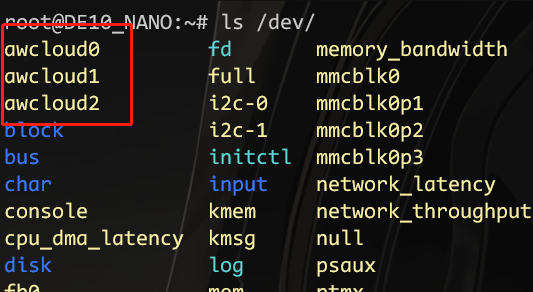
\includegraphics[width=\linewidth]{multi_devices.png}
  \caption{驱动的多设备管理}
  \label{fig:multi_devices}
\end{figure}

\section{Platform驱动模型}

\chapter{Linux系统编程}

\section{Linux文件系统udev}
Udev工作在用户态,其基本的原理是利用设备插入或者移除时,内核所发送的热插拔
事件进行工作的。热插拔时,设备的详细信息会由内核通过netlink套接字发送uevent
时间信息。而udev的设备命名,权限和时间处理都是在用户态下完成的,利用的就是内核
收到的信息进行设备文件节点的创建和删除操作。如下代码所示:
\begin{code-block}{c}
#include <poll.h>
#include <stdio.h>
#include <string.h>
#include <unistd.h>
#include <sys/socket.h>
#include <linux/netlink.h>

int main(int argc, char * argv[])
{
        struct sockaddr_nl nls;
        struct pollfd pfd;
        char buffer[1024];

        memset(&nls, 0, sizeof(struct sockaddr_nl));
        nls.nl_family = AF_NETLINK;
        nls.nl_pid = getpid();
        nls.nl_groups = -1;

        pfd.events = POLLIN;
        pfd.fd = socket(AF_NETLINK, SOCK_DGRAM, NETLINK_KOBJECT_UEVENT);

        if (-1 == pfd.fd) {
                printf("ERROR: not root\n");
                return -1;
        }

        if (bind(pfd.fd, (void*)&nls, sizeof(struct sockaddr_nl))) {
                printf("ERROR: bind failed\n");
                return -1;
        }

        while ( -1 != poll(&pfd, 1, -1)) {
                int i, len = recv(pfd.fd, buffer, 1024, MSG_DONTWAIT);
                if (-1 == len) {
                        printf("Recv Nothing\n");
                        return -1;
                }

                i = 0;
                while (i < len) {
                        printf("%s\n", buffer+i);
                        i += strlen(buffer + i) + 1;
                }
        }

        printf("POLL \n");

        return 0;
}
\end{code-block}
执行上述的程序,当内核监听到存在设备的变更时,就会自动的提示相关的信息。在linux
系统当中,也可以直接使用指令进行udev设备变更的监听:
\begin{code-block}{bash}
udevadm monitor --kernel --property --udev
\end{code-block}

\section{IO函数}
Linux系统当中,通常需要处理IO,而IO的处理,在Linux的函数当中,主要有4个函数:
\begin{itemize}
  \item open //fcntl.h
  \item write //unistd.h
  \item read //unistd.h
  \item close //unistd.h
\end{itemize}

实现简单的touch命令的功能
\begin{code-block}{c}
#include <stdio.h>
#include <unistd.h>
#include <fcntl.h>

int main(int argc, char * argv[])
{
        // 第3个参数可以直接写为0644
        int fd = open(argv[1], O_CREAT|O_WRONLY,
                S_IRUSR|S_IWUSR|S_IRGRP|S_IROTH);
        if (0>fd)
        {
                printf("Cannot create file %s\n", argv[1]);
                return -1;
        }
        printf("Create file %s success\n", argv[1]);
        close(fd);
        return 0;
}
\end{code-block}

但是,由于Linux操作系统本身存在umask(默认为022),因此,如果上述的第3个参数写作0777,
生成的文件的权限与umask进行亦或计算之后,实际上,文件的权限还是755,并不是我们所期待的
777。如果需要保持设置的权限与生成的文件权限完全一致,需要执行如下命令:
\begin{code-block}{bash}
umask 000
# 后续再执行代码,生成文件
\end{code-block}

Open函数只能生成普通文件,如果是管道、字符设备之类的,则无法使用open函数进行创建。
另外,如果只是需要打开文件,并不是创建文件,则open函数的第3个参数不需要。
除此之外,还需要注意一下,文件的打开模式
\begin{itemize}
  \item O\_TRUNC:覆盖文件
  \item O\_EXCL : 与O\_CREAT合用,如果对应文件已经存在,则提示错误
\end{itemize}

Open函数一旦调用,Linux内核会在内核空间打开3个文件描述符,分别是0,1,2。

而对应的,也可以利用write函数向打开的文件句柄当中写入内容
\begin{code-block}{c}
#include <stdio.h>
#include <unistd.h>
#include <fcntl.h>

int main(int argc, char * argv[])
{
        // 第3个参数可以直接写为0644
        int fd = open(argv[1], O_CREAT|O_RDWR,
                S_IRUSR|S_IWUSR|S_IRGRP|S_IROTH);
        if (0>fd)
        {
                printf("Cannot create file %s\n", argv[1]);
                return -1;
        }
        printf("Create file %s success\n", argv[1]);

        char msg[] = "hello world";
        write(fd, msg, sizeof(msg)/sizeof(char)); //会写入一个文件结束符,特殊符号
                                                  // 如果不需要,则将长度-1即可
        close(fd);
        return 0;
}
\end{code-block}

相应的,也可以利用read函数读取打开文件的内容:
\begin{code-block}{c}
#include <stdio.h>
#include <unistd.h>
#include <fcntl.h>
#include <string.h>

int main(int argc, char * argv[])
{
        int fd = open(argv[1], O_RDONLY);
        if (0>fd)
        {
                printf("Cannot open file %s\n", argv[1]);
                return -1;
        }
        printf("Open file %s success\n", argv[1]);

        size_t read_ret = 0;
#if 0
        // 连续多次读取,并非一次性读完
        size_t total = 0;
        char readbuf[128];
        while ((read_ret=read(fd, readbuf, 127))>0) // 每次只能读取max-1,否则末尾存在特殊字符,可能出现溢出
        {
                total += read_ret;
                printf("Read %d chars \n", read_ret);
                printf("The content of file is %s \n", readbuf);
                memset(readbuf, 0, 128);
        }
        printf("The total sizeof file is %d\n", total);
#else
        // 一次性读取
        char readbuf[1024];
        read_ret=read(fd, readbuf, 1024);
        printf("Read %d chars \n", read_ret);
        printf("The content of file is %s \n", readbuf);
#endif
        close(fd);
        return 0;
}
\end{code-block}

高级一点的,我们就可以使用read和write函数来实现一个简单的文件拷贝功能。
\begin{code-block}{c}
#include <stdio.h>
#include <unistd.h>
#include <fcntl.h>
#include <string.h>

int main(int argc, char * argv[])
{
        int readrd = 0, writefd = 0;
        if (0 >= (readrd = open(argv[1], O_RDONLY)))
        {
                printf("Cannot open the source file %s\n", argv[1]);
                return -1;
        }
        if (0 >= (writefd = open(
                argv[2], O_CREAT|O_TRUNC|O_WRONLY, 0644)))
        {
                printf("Cannot create the target file %s\n", argv[2]);
                return -1;
        }

        unsigned char buffer[128];
        memset(buffer, 0, 128);

        size_t readret = 0, writeret = 0;
        while(0 < (readret = read(readrd, buffer, 127)))
        {
                if (0 > (writeret = write(writefd, buffer, readret)))
                {
                        printf("Cannot write content to write file\n");
                        return -1;
                }
                memset(buffer, 0, 128);
        }

        close(readrd);
        close(writefd);
        return 0;
}
\end{code-block}

由于读取使用的是unsigned char,因此,上述文件也可以直接拷贝二进制文件。
\section{文件属性}
每一个文件都存在属性,所谓的属性,包含了文件的打开状态,访问模式等等。而判断这些属性,则需要使用fcntl函数。
该函数的使用比较广泛,可以从各个层面来判断文件的状态和模式,参见下列代码:
\begin{code-block}{c}
#include <unistd.h>
#include <fcntl.h>
...
        int fd = 0;
        int flags = 0;
        int access_mode = 0;
        // 获取文件的打开状态
        if (-1 == (flags = fcntl(fd, F_GETFL))) {
                printf("Cannot get the file flags\n");
                goto fcntl_err;
        }

        // 判断文件的状态,是否已同步的方式打开
        if (flags & O_SYNC) {
                printf("File opened in sync mode\n");
        }

        // 获取并判断文件的访问模式
        if ( O_RDONLY == (access_mode = (flags & O_ACCMODE))) {
                printf("File is opened with read_only mode\n");
        }

        // 修改文件的状态
        flags |= O_APPEND;
        if ( -1 == (flags = fcntl(fd, F_SETFL, flags))) {
                printf("Cannot set the file flags\n");
                goto fcntl_err;
        }
...
\end{code-block}

\section{标准IO函数}
Linux的IO操作包括文件IO和标准IO。所谓的文件IO,即直接调用内核提供的系统调用函数,一般需要使用头文件unistd.h当中的函数;而
标准IO,则是通过调用C的库函数,间接的调用系统调用函数,通常的,使用的头文件stdio.h当中的函数。从功能上看,标准IO与文件IO是
相同的,但是,细节上,他们存在区别。
\begin{code-block}{c}
#include <stdio.h>
#include <unistd.h>

int main(int argc, char * argv[])
{
        char  buffer[] = "hello world";
        printf("stdio %s", buffer);
        write(1, buffer, 11);
        while(1);
        return 0;
}
\end{code-block}

上述代码编译之后,运行,只有hello world能够输出,而printf的stdio hello world则无法输出。问题在于缓存。
Linux程序当中存在几种缓存:
\begin{itemize}
  \item 用户空间缓存:即想从内核读写的数据,即上述代码当中buffer
  \item 内核空间缓存:没打开一个文件,内核会在内核空间开辟一块缓存,这个称之为内核空间的缓存
  \item 库缓存:标准IO的库函数的缓存
\end{itemize}

文件IO中的写,即是将用户空间的缓存写入到内核空间缓存当中;反之,文件IO的读,则是将内核空间的缓存读写到用户空间的缓存当中。
而调用标准IO之后,数据会从用户空间写入到库缓存,当写入的数据包含\textbackslash n时,或者库缓存空间写满时,才会向内核缓存空间提交数据。
因此,如果上述代码修改为
\begin{code-block}{c}
printf("stdio %s\n", buffer); //或者直接将库缓存写满
while(1);
\end{code-block}
则会直接输出。另外,库缓存的大小默认为1024个字节。

常用fgets,gets,printf,sprintf,fprintf,fputs,puts,scanf这些函数在遇到\textbackslash n或者写满缓存时,即
调用系统调用函数,称之为行缓存函数;而fread,fwrite只有在写满缓存之后再调用系统调用函数,这些则称之为全缓存函数;
而只要调用,则会将内容和数据写入到内核当中的函数,称之为无缓存函数,注意,stderr是无缓存的,而stdout则是行缓存的。
fclose函数在关闭文件之前,会刷新缓存当中的数据到文件当中。

需要注意的是fputc是缓存函数,但是,他不是行缓存函数,立即生效的话,需要使用fflush函数进行强制刷新。

除此之外,在标准IO当中,读取文件有可能会出现错误,而fgets函数读取正常时,返回读取到的内容,这个内容与fgets函数的第一个参数的结果一致,
如果读取错误,则会返回一个空指针(char)。但是无法准确判断这个错误是什么类型。判断错误的准确类型,可以使用feof和ferror函数进行判断。
前者表示读取到了文件末尾,而后一个则表示真的文件读取错误,如下代码所示:
\begin{code-block}{c}
FILE *fp = fopen("test.c")
char buffer[128];
char * read_ret = NULL;
read_ret = fgets(buffer, 128, fp);
if (NULL == read_ret)
{
        if(feof(fp))
        {
                printf("Read the end of file\n");
        }
        if(ferror(fp))
        {
                printf("Read error from the stream\n");
        }
}
\end{code-block}

与文件IO相对应的,标准IO使用fopen函数进行文件的创建和读写。但是需要特别注意的是,实际上,fopen函数创建的函数的权限始终是
666,但是由于umask的存在,因此,fopen函数创建的文件的最终权限为644。

全缓存函数fread和fwrite在使用的时候会调用syscall,写入到内核缓存当中,最后写入到硬件当中(文件)。同样的,我们也可以用fread和fwrite实现
Linux的cat命令,简单的如下:
\begin{code-block}{c}
if(NULL == (fp = fopen(argv[1], "rb")))
{
        printf("Cannot open the file %s\n", argv[1]);
        return -1;
}

unsigned char buffer[128];
memset(buffer, 0, 128);
while(0 < fread(buffer, sizeof(char), 128, fp))
{
        fwrite(buffer, sizeof(char), 128, stdout);
        memset(buffer, 0, 128);
        if(feof(fp))
        {
                printf("Read the the of file\n");
                break;
        }
}

fclose(fp); // 调用fflush,直接写入到内核缓存当中
return 0;
\end{code-block}

从执行效率上说,fgetc/fputc<fgets/fputs<fread/fwrite,主要原因在于fread基本都是在内核空间操作,效率有保证。因此,在有高效率要求的情况下,尽可能的使用fread和fwrite
作为IO的操作函数。

\section{目录IO}
除了文件IO和标准IO之外,Linux还提供了针对路径(目录)的IO操作函数,具体如图\colorunderlineref{fig:dirio}所示
\begin{figure}[H]
  \centering
  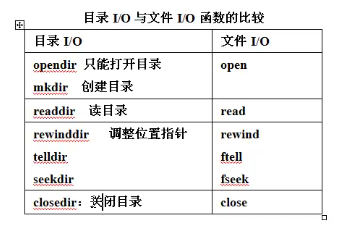
\includegraphics[width=\linewidth]{dirio.png}
  \caption{Linux的目录IO函数}
  \label{fig:dirio}
\end{figure}

只是需要注意的是,mkdir函数在sys/stat.h当中,其他的函数大部分在dirent.h当中。目录的创建,可以使用如下的代码:
\begin{code-block}{c}
int ret = mkdir("zhangjl", 0777);
if(0 > ret)
{
        printf("Failed to create dir\n");
        return -1;
}
return 0;
\end{code-block}

而打开目录,则可以如下操作:
\begin{code-block}{c}
#include <dirent.h>

int main(int argc, char * argv[])
{
        DIR *dp = opendir("/root");
        if(NULL ==  dp)
        {
                printf("Failed to open dir\n");
                return -1;
        }

        closedir(dp);
        return 0;
}
\end{code-block}

读取目录内容,则可以使用readdir函数。由于readdir函数在多个头文件当中都有定义,此处应当使用dirent.h当中的函数。
具体的使用如下代码:
\begin{code-block}{c}
#include <stdio.h>
#include <dirent.h>

int main(int argc, char * argv[])
{
        DIR *dp = opendir("/root/cprograms/dirio");
        if(NULL ==  dp)
        {
                printf("Failed to open dir\n");
                return -1;
        }

        struct dirent * dir = NULL;
        while (NULL != (dir = readdir(dp)))
        {
                printf("The inode is %lu, and name is %s\n",
                        dir->d_ino, dir->d_name);
        }

        closedir(dp);
        return 0;
}
\end{code-block}
上述代码需要注意的有几点:
\begin{enumerate}
  \item readdir返回的是一个指针,而这个指针,实际上是一个链表的头指针,因此,通常情况下需要反复调用该函数,读取链表上的所有元素
  \item readdir只能返回一级文件目录当中的内容,子目录以及子目录下的子目录,则无法一次性读取
  \item rewinddir则会将readdir所得到的指针,重新定位到这个链表的头节点,也可以使用seekdir进行指定地址的跳转。
\end{enumerate}

\section{Linux进程通信}
Linux常见的进程间通信模式主要如下:
\begin{itemize}
    \item 管道pipe

            管道是一种半双工的通信方式,数据只能单向流动,而且只能在具有亲缘关系的进程间使用。进程的亲缘关系通常是指父子进程关系。
    \item 命名管道FIFO

            有名管道也是半双工的通信方式,但是它允许无亲缘关系进程间的通信。
    \item 消息队列MessageQueue

            消息队列是由消息的链表,存放在内核中并由消息队列标识符标识。消息队列克服了信号传递信息少、管道只能承载无格式字节流以及缓冲区大小受限等缺点。
    \item 共享存储SharedMemory

            共享内存就是映射一段能被其他进程所访问的内存,这段共享内存由一个进程创建,但多个进程都可以访问。共享内存是最快的 IPC 方式,它是针对其他进程间通信方式运行效率低而专门设计的。它往往与其他通信机制,如信号两,配合使用,来实现进程间的同步和通信。
    \item 信号量Semaphore

            信号量是一个计数器,可以用来控制多个进程对共享资源的访问。它常作为一种锁机制,防止某进程正在访问共享资源时,其他进程也访问该资源。因此,主要作为进程间以及同一进程内不同线程之间的同步手段。
    \item 套接字Socket

            套解口也是一种进程间通信机制,与其他通信机制不同的是,它可用于不同及其间的进程通信。
    \item 信号 ( sinal )

            信号是一种比较复杂的通信方式,用于通知接收进程某个事件已经发生。
\end{itemize}

\subsection{管道方式}
管道,通常指无名管道,是 UNIX 系统IPC最古老的形式。
\begin{itemize}
    \item 半双工

            数据只能在一个方向上流动,具有固定的读端和写端。
    \item 亲缘关系

            只能用于具有亲缘关系的进程之间的通信(也是父子进程或者兄弟进程之间)。
    \item 特殊文件

            对于它的读写也可以使用普通的read、write 等函数。但是它不是普通的文件,并不属于其他任何文件系统,并且只存在于内存中。
\end{itemize}

当一个管道建立时,它会创建两个文件描述符:fd[0]为读而打开,fd[1]为写而打开。如下图:\colorunderlineref{fig:pipe}
\begin{figure}[H]
  \centering
  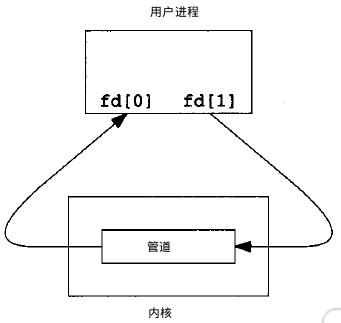
\includegraphics[width=\linewidth]{pipe.png}
  \caption{管道}
  \label{fig:pipe}
\end{figure}
需要注意的是,fd[0]永远用于读取,不管是子进程还是父进程,都只能从fd[0]读取;fd[1]永远用于写入,子进程和父进程都只能从
fd[1]写入。如果fd的使用搞反,则会导致消息无法正常传递。

单个进程中的管道几乎没有任何用处。所以,通常调用 pipe 的进程接着调用 fork,这样就创建了父进程与子进程之间的 IPC 通道。如下图所示:\colorunderlineref{fig:fork_pipe}
\begin{figure}[H]
  \centering
  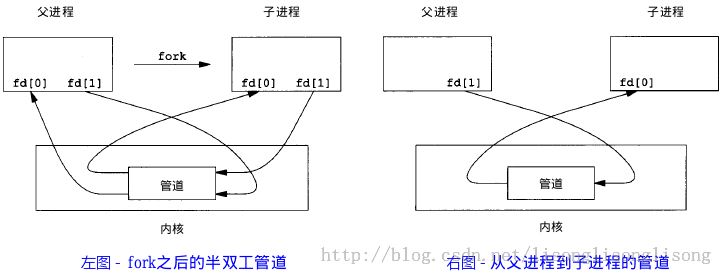
\includegraphics[width=\linewidth]{fork_pipe.png}
  \caption{fork管道}
  \label{fig:fork_pipe}
\end{figure}

使用管道的具体方式如下:
\begin{code-block}{c}
#include <stdio.h>
#include <unistd.h>

int main(int argc, char * argv[])
{
        int fd[2];
        pid_t pid;
        char buf[20];

        if(0 > pipe(fd))
        {
                printf("Create Pipe Error!\n");
                return -1;
        }
        if(0 > (pid = fork()))
        {
                printf("Fork error\n");
                return -1;
        }
        if(0 == pid)
        {
#if 1
                // 父进程接收
                close(fd[1]);
                read(fd[0], buf, 20);
                printf("%s in pid %d\n", buf, pid);
                close(fd[0]);
#else
                // 父进程输入
                printf("pid: %d\n", pid);
                close(fd[0]);
                write(fd[1], "Hello World\n", 12);
                close(fd[1]);
#endif
        }
        else{
#if 1
                // 子进程输入
                printf("pid: %d\n", pid);
                close(fd[0]);
                write(fd[1], "Hello World\n", 12);
                close(fd[1]);
#else
                // 子进程接收
                close(fd[1]);
                read(fd[0], buf, 20);
                printf("%s in pid %d\n", buf, pid);
                close(fd[0]);
#endif
        }
        return 0;
}
\end{code-block}

\subsection{命名管道FIFO}
FIFO,也称为命名管道,它是一种文件类型。FIFO可以在无关的进程之间交换数据,与无名管道不同。FIFO有路径名与之相关联,它以一种特殊设备文件形式存在于文件系统中。
通常使用mkfifo创建一个命名管道。一旦创建了一个 FIFO,就可以用一般的文件I/O函数操作它。FIFO的通信方式类似于在进程中使用文件来传输数据,只不过FIFO类型文件同时具有管道的特性。
在数据读出时,FIFO管道中同时清除数据,并且“先进先出”。
下面的例子演示了使用 FIFO 进行 IPC 的过程。
Server端负责创建fifo,并保持监听。
\begin{code-block}{c}
// server.c
#include <stdio.h>
#include <stdlib.h>
#include <fcntl.h>
#include <errno.h>
#include <sys/stat.h>
#include <unistd.h>
#include <signal.h>

#define FIFO_PATH "/tmp/fifo"
static int fd = -1;
static void ctrl_c(int sig);

static inline void clean()
{
        if(0 < fd)
        {
                close(fd);  // 关闭FIFO文件
        }
        remove(FIFO_PATH);
}

int main(int argc, char * argv[])
{
        int len;
        char buf[1024];

        if (SIG_ERR == signal(SIGINT, ctrl_c))
        {
                printf("\ncan't catch SIGINT\n");
                goto finally;
        }

        if(mkfifo(FIFO_PATH, 0666) < 0 && errno!=EEXIST) // 创建FIFO管道
                perror("Create FIFO Failed");

        if((fd = open(FIFO_PATH, O_RDONLY)) < 0)  // 以读打开FIFO
        {
                perror("Open FIFO Failed");
                exit(1);
        }

        while(1)
        {
                len = read(fd, buf, 1024);
                if (0 < len)
                {
                        printf("Read message: %s", buf);
                }
                else if (0 > len)
                {
                        perror("Unexpected error\n");
                        break;
                }
        }

finally:
        clean();
        return 0;
}

void ctrl_c(int sig)
{
        if (SIGINT == sig)
        {
                printf("Recevied ctrl+c interrupt, try to clean the env\n");
                clean();
                exit(0);
        }
}
\end{code-block}

Client端负责连接fifo,并通过fifo进行通信。
\begin{code-block}{c}
// client.c
#include <stdio.h>
#include <stdlib.h>   // exit
#include <fcntl.h>    // O_WRONLY
#include <sys/stat.h>
#include <time.h>     // time
#include <unistd.h>

#define FIFO_PATH "/tmp/fifo"

int main(int argc, char * argv[])
{
        int fd;
        int n, i;
        char buf[1024];
        time_t tp;
        printf("I am %d process.\n", getpid()); // 说明进程ID

        if((fd = open(FIFO_PATH, O_WRONLY)) < 0) // 以写打开一个FIFO
        {
                perror("Open FIFO Failed");
                exit(1);
        }
        for(;;)
        {
                time(&tp);  // 取系统当前时间
                n=sprintf(buf,"Process %d's time is %s",getpid(),ctime(&tp));
                printf("Send message: %s", buf); // 打印
                if(write(fd, buf, n+1) < 0)  // 写入到FIFO中
                {
                        perror("Write FIFO Failed");
                        close(fd);
                        exit(1);
                }
                sleep(1);  // 休眠1秒
        }
        close(fd);  // 关闭FIFO文件
        return 0;
}
\end{code-block}

稍微特殊的情况是,在server端的代码中,加入了对ctrl+c的中断识别操作,确保server端可以执行对应的扫尾工作。本身对ctrl+c的中断
操作属于信号量和中断的范畴。上述例子可以展成客户进程—服务器进程通信的实例,可以打开多个客户端
向一个服务器发送请求信息,server端实时监控着FIFO的读端,
在之后的内容会有更加详细的讲解。当有数据时,读出并进行处理,但是有一个关键的问题是,
每一个客户端必须预先知道服务器提供的FIFO接口,下图显示了这种安排\colorunderlineref{fig:fifo}
\begin{figure}[H]
  \centering
  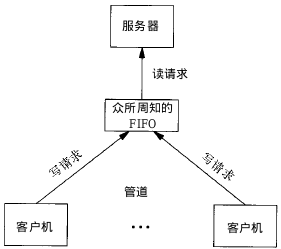
\includegraphics[width=\linewidth]{fifo.png}
  \caption{FIFO管道}
  \label{fig:fifo}
\end{figure}

\subsection{消息队列}
消息队列,是消息的链接表,存放在内核中。一个消息队列由一个标识符(即队列ID)来标识。

消息队列拥有自己的一些特点:
\begin{itemize}
    \item 消息队列是面向记录的,其中的消息具有特定的格式以及特定的优先级。
    \item 消息队列独立于发送与接收进程。进程终止时,消息队列及其内容并不会被删除。
    \item 消息队列可以实现消息的随机查询,消息不一定要以先进先出的次序读取,也可以按消息的类型读取。
\end{itemize}

消息队列的主要原型在如下的头文件当中:
\begin{code-block}{c}
#include <sys/msg.h>
// 创建或打开消息队列:成功返回队列ID,失败返回-1
int msgget(key_t key, int flag);
// 添加消息:成功返回0,失败返回-1
int msgsnd(int msqid, const void *ptr, size_t size, int flag);
// 读取消息:成功返回消息数据的长度,失败返回-1
int msgrcv(int msqid, void *ptr, size_t size, long type,int flag);
// 控制消息队列:成功返回0,失败返回-1
int msgctl(int msqid, int cmd, struct msqid_ds *buf);
\end{code-block}

在以下两种情况下,msgget将创建一个新的消息队列:
\begin{itemize}
    \item 如果没有与键值key相对应的消息队列,并且flag中包含了IPC\_CREAT标志位。
    \item key参数为IPC\_PRIVATE
\end{itemize}

函数msgrcv在读取消息队列时,type参数有下面几种情况:
\begin{itemize}
    \item type == 0,返回队列中的第一个消息
    \item type > 0,返回队列中消息类型为 type 的第一个消息
    \item type < 0,返回队列中消息类型值小于或等于 type 绝对值的消息,如果有多个,则取类型值最小的消息
\end{itemize}

可以看出,type值非0时用于以非先进先出次序读消息。也可以把type看做优先级的权值。
下面的例子使用消息队列进行IPC,服务端程序一直在等待特定类型的消息,当收到该类型的
消息以后,发送另一种特定类型的消息作为反馈,客户端读取该反馈并打印出来。
\begin{code-block}{c}
// server.c
#include <stdio.h>
#include <stdlib.h>
#include <sys/msg.h>
#include <unistd.h>

// 用于创建一个唯一的key
#define MSG_FILE "/etc/passwd"

// 消息结构
struct msg_form {
        long mtype;
        char mtext[256];
};

int main()
{
        int msqid;
        key_t key;
        struct msg_form msg;
        // 获取key值
        // 只有server端和client端获得的key相同,server端和client端才能进行通信
        if((key = ftok(MSG_FILE,'z')) < 0)
        {
                perror("ftok error");
                exit(1);
        }

        // 打印key值
        printf("Message Queue - Server key is: %d.\n", key);

        // 创建消息队列
        if ((msqid = msgget(key, IPC_CREAT|0777)) == -1)
        {
                perror("msgget error");
                exit(1);
        }

        // 打印消息队列ID及进程ID
        printf("My msqid is: %d.\n", msqid);
        printf("My pid is: %d.\n", getpid());

        // 循环读取消息
        for(;;)
        {
                msgrcv(msqid, &msg, 256, 888, 0);// 返回类型为888的第一个消息
                printf("Server: receive msg.mtext is: %s.\n", msg.mtext);
                printf("Server: receive msg.mtype is: %d.\n", msg.mtype);

                msg.mtype = 999; // 客户端接收的消息类型
                sprintf(msg.mtext, "hello, I'm server %d", getpid());
                msgsnd(msqid, &msg, sizeof(msg.mtext), 0);
        }
        return 0;
}
\end{code-block}

而客户端的代码有区别
\begin{code-block}{c}
// client.c
#include <stdio.h>
#include <stdlib.h>
#include <sys/msg.h>
#include <unistd.h>

// 用于创建一个唯一的key
#define MSG_FILE "/etc/passwd"

// 消息结构
struct msg_form {
        long mtype;
        char mtext[256];
};

int main()
{
        int msqid;
        key_t key;
        struct msg_form msg;

        // 获取key值
        if ((key = ftok(MSG_FILE, 'z')) < 0)
        {
                perror("ftok error");
                exit(1);
        }

        // 打印key值
        printf("Message Queue - Client key is: %d.\n", key);

        // 打开消息队列
        if ((msqid = msgget(key, IPC_CREAT|0777)) == -1)
        {
                perror("msgget error");
                exit(1);
        }

        // 打印消息队列ID及进程ID
        printf("My msqid is: %d.\n", msqid);
        printf("My pid is: %d.\n", getpid());

        // 添加消息,类型为888
        msg.mtype = 888;
        sprintf(msg.mtext, "hello, I'm client %d", getpid());
        msgsnd(msqid, &msg, sizeof(msg.mtext), 0);

        // 读取类型为999的消息
        msgrcv(msqid, &msg, 256, 999, 0);
        printf("Client: receive msg.mtext is: %s.\n", msg.mtext);
        printf("Client: receive msg.mtype is: %d.\n", msg.mtype);
        return 0;
}
\end{code-block}

比较有意思的是,内核的消息队列和真正的消息队列服务器行为一致。当消息发出,没有接收者
时,依然会存在消息积压,只不过这些消息是积压在内核空间的。当接收者出现之后,这些
积压在内核空间的消息,还是会被正确投递。

\subsection{信号量}
信号量(semaphore)与已经介绍过的IPC结构不同,它是一个计数器。信号量用于实现进程间的互斥与同步,而不是用于存储进程间通信数据。
\begin{itemize}
    \item 信号量用于进程间同步,若要在进程间传递数据需要结合共享内存。
    \item 信号量基于操作系统的PV操作,程序对信号量的操作都是原子操作
    \item 每次对信号量的PV操作不仅限于对信号量值加1或减1,而且可以加减任意正整数。
    \item 支持信号量组。
\end{itemize}

最简单的信号量是只能取0和1的变量,这也是信号量最常见的一种形式,叫做二值信号量(Binary Semaphore)。而可以取多个正整数的信号量被称为通用信号量。
Linux下的信号量函数都是在通用的信号量数组上进行操作,而不是在一个单一的二值信号量上进行操作。实际应用时,我们每次都需要创建一个信号量集,
即使此集合只包含一个信号量。一般我们通过下面函数去创建或者打开一个信号量集。
\begin{code-block}{c}
int semget(key_t key,int nsems,int semflg);
\end{code-block}

当semflg=IPC\_CREATE时,如果当前系统中不存在此信号量集合(key值不存在),
那么semget函数完成一个信号量的创建;否则,semget函数打开这个已存在的信号量集。
当semflg=IPC\_CREATE|IPC\_EXCL时,只会完成创建,如果key值对应的信号量集合以存在,
那么直接返回错误,错误代码为EEXIST。这并不难理解,和open文件的情况类似。此函数
成功执行返回信号量集的标示符,否则为-1。

而常用的信号量函数如下:
\begin{code-block}{c}
#include <sys/sem.h>
// 创建或获取一个信号量组:若成功返回信号量集ID,失败返回-1
int semget(key_t key, int num_sems, int sem_flags);
// 对信号量组进行操作,改变信号量的值:成功返回0,失败返回-1
int semop(int semid, struct sembuf semoparray[], size_t numops);
// 控制信号量的相关信息
int semctl(int semid, int sem_num, int cmd, ...);
\end{code-block}

当semget创建新的信号量集合时,必须指定集合中信号量的个数(即num\_sems),通常为1;
如果是引用一个现有的集合,则将sems\_num指定为 0 。sembuf结构的定义如下:
\begin{code-block}{c}
struct sembuf
{
    short sem_num; // 信号量组中对应的序号,0~sem_nums-1
    short sem_op;  // 信号量值在一次操作中的改变量
    short sem_flg; // IPC_NOWAIT, SEM_UNDO
}
\end{code-block}

通过semid和sem\_num两个字段就可以确定信号量集中的指定信号量。sem\_op取不同的值就会
产生不同的操作。特别的,如果其值为0,则此时sem\_op操作的作用是测试信号量的值是否为0。
sem\_op是一次操作中的信号量的改变量,若sem\_op > 0,表示进程释放相应的资源数,将
sem\_op的值加到信号量的值上。如果有进程正在休眠等待此信号量,则唤醒他们。

若sem\_op < 0,请求sem\_op的绝对值的资源,如果相应的资源数可以满足请求,则将该信号量的值减去sem\_op的绝对值,
函数成功返回。当相应的资源数不能满足请求时,这个操作与sem\_flg有关。sem\_flg 指定IPC\_NOWAIT,则semop函数出错
返回EAGAIN。sem\_flg 没有指定IPC\_NOWAIT,则将该信号量的semncnt值加1,然后进程挂起直到下述情况发生:当相应的
资源数可以满足请求,此信号量的semncnt值减1,该信号量的值减去sem\_op的绝对值。成功返回;此信号量被删除,函数
smeop出错返回EIDRM;进程捕捉到信号,并从信号处理函数返回,此情况下将此信号量的semncnt值减1,函数semop出错
返回EINTR。

若sem\_op==0,进程阻塞直到信号量的相应值为0:当信号量已经为0,函数立即返回。如果信号量的值不为0,则依据
sem\_flg决定函数动作:sem\_flg指定IPC\_NOWAIT,则出错返回EAGAIN。sem\_flg没有指定IPC\_NOWAIT,则将该信号量的
semncnt值加1,然后进程挂起直到下述情况发生:信号量值为0,将信号量的semzcnt的值减1,函数semop成功返回;此
信号量被删除,函数smeop出错返回EIDRM;进程捕捉到信号,并从信号处理函数返回,在此情况将此信号量的semncnt值
减1,函数semop出错返回EINTR。

在semctl函数中的命令有多种,这里就说两个常用的:SETVAL:用于初始化信号量为一个已知的值。所需要的值作为联合
semun的val成员来传递。在信号量第一次使用之前需要设置信号量。IPC\_RMID:删除一个信号量集合。如果不删除信号量,
它将继续在系统中存在,即使程序已经退出,它可能在你下次运行此程序时引发问题,而且信号量是一种有限的资源。

一个简单的例子。如果不使用信号量,父进程会先于子进程输出。但是,使用信号量之后,子进程会先于父进程执行。
\begin{code-block}{c}
#include <stdio.h>
#include <stdlib.h>
#include <sys/sem.h>
#include <unistd.h>

union semun
{
        int              val; /*for SETVAL*/
        struct semid_ds *buf;
        unsigned short  *array;
};

// 初始化信号量
int init_sem(int sem_id, int value)
{
        union semun tmp;
        tmp.val = value;
        if(semctl(sem_id, 0, SETVAL, tmp) == -1)
        {
                perror("Init Semaphore Error");
                return -1;
        }
        return 0;
}

// P操作:
//    若信号量值为1,获取资源并将信号量值-1
//    若信号量值为0,进程挂起等待
int sem_p(int sem_id)
{
        struct sembuf sbuf;
        sbuf.sem_num = 0; /*序号*/
        sbuf.sem_op = -1; /*P操作*/
        sbuf.sem_flg = SEM_UNDO;

        if(semop(sem_id, &sbuf, 1) == -1)
        {
                perror("P operation Error");
                return -1;
        }
        return 0;
}

// V操作:
//    释放资源并将信号量值+1
//    如果有进程正在挂起等待,则唤醒它们
int sem_v(int sem_id)
{
        struct sembuf sbuf;
        sbuf.sem_num = 0; /*序号*/
        sbuf.sem_op = 1;  /*V操作*/
        sbuf.sem_flg = SEM_UNDO;

        if(semop(sem_id, &sbuf, 1) == -1)
        {
                perror("V operation Error");
                return -1;
        }
        return 0;
}

// 删除信号量集
int del_sem(int sem_id)
{
        union semun tmp;
        if(semctl(sem_id, 0, IPC_RMID, tmp) == -1)
        {
                perror("Delete Semaphore Error");
                return -1;
        }
        return 0;
}


int main()
{
        int sem_id;  // 信号量集ID
        key_t key;
        pid_t pid;

        // 获取key值
        if((key = ftok(".", 'z')) < 0)
        {
                perror("ftok error");
                exit(1);
        }

        // 创建信号量集,其中只有一个信号量
        if((sem_id = semget(key, 1, IPC_CREAT|0666)) == -1)
        {
                perror("semget error");
                exit(1);
        }

        // 初始化:初值设为0资源被占用
        init_sem(sem_id, 0);

        if((pid = fork()) == -1)
                perror("Fork Error");
        else if(pid == 0) /*子进程*/
        {
                //sleep(2);
                printf("Process child: pid=%d\n", getpid());
                sem_v(sem_id);  /*释放资源*/
        }
        else  /*父进程*/
        {
                sem_p(sem_id);   /*等待资源*/
                printf("Process father: pid=%d\n", getpid());
                sem_v(sem_id);   /*释放资源*/
                del_sem(sem_id); /*删除信号量集*/
        }
        return 0;
}
\end{code-block}
首先需要明确的是,在用户空间实现进程间通信是不可能的,需要在Linux内核空间当中进行;但是线程间的通信,在用户空间就可以实现。
最明显的,线程间的通信,通过全局变量即可实现,其原因主要就是多线程之间是共享内存的,如下简单代码:
\begin{code-block}{c}
#include <stdio.h>
#include <pthread.h>
#include <unistd.h>
int main_run = 0;
void *func(void *var)
{
        int i = 0;
        //while(!main_run); //如果需要父进程执行结束之后,再执行子线程,则开启本行注释即可
        for (; i <10; i++)
        {
                usleep(100);
                printf("This is fun i=%d\n", i);
        }
}

int main(int argc, char * argv[])
{
        int i = 0;
        char buf[] = "hello world\n";
        pthread_t tid;
        int ret = 0;
        ret = pthread_create(&tid, NULL, func, (void*)buf);
        if (0 > ret)
        {
                printf("Create thread failure\n");
                return -1;
        }
        for(i = 0; i < 10; i++)
        {
                usleep(100);
                printf("this is main fun i = %d\n", i);
        }
        main_run = 1;
        while(1);
        return 0;
}
\end{code-block}

注意,多线程编译时,需要加入-pthread参数,即
\begin{code-block}{bash}
gcc -pthread -o test test.c
\end{code-block}

但是,与线程不同,进程间的每一种通信方式都是基于文件IO的思想进行设计和实现的。

\subsection{管道通信}
管道是一种特殊的文件,由队列来实现,遵循先进先出的顺序。与open函数类似,open函数打开的文件描述符为0,1,2,而管道函数(pipe)
打开的文件描述符则固定为3,4,分别对应fd[0]和fd[1]。在内核当中,管道实际上是使用数组进行实现的。
\begin{code-block}{c}
#include <stdio.h>
#include <unistd.h>

int main(int argc, char * argv[])
{
        int fd[2];
        int ret = 0;
        if (0 > (ret=pipe(fd)))
        {
                printf("Cannot create pipe \n");
                return -1;
        }
        printf("%d, %d\n", fd[0], fd[1]);
        return 0;
}
\end{code-block}

由于管道本身是特殊文件,因此,也可以对管道进行读写,但是特别需要注意的是,fd[0]只允许进行读取,而fd[1]则只允许进行写入,如下:
\begin{code-block}{c}
#include <stdio.h>
#include <unistd.h>
#include <string.h>

int main(int argc, char * argv[])
{
        int fd[2];
        int ret = 0;
        if (0 > (ret=pipe(fd)))
        {
                printf("Cannot create pipe \n");
                return -1;
        }
        char buf[] = "hello linux";
        char readbuf[128];
        memset(readbuf, 0, 128);
        size_t writed = write(fd[1], buf, sizeof(buf)/sizeof(char));
        size_t readed = read(fd[0], readbuf, writed);
        printf("Read from pipe: %s\n", readbuf);
        close(fd[0]);
        close(fd[1]);
        return 0;
}
\end{code-block}

\begin{enumerate}
  \item 管道创建在内存当中,进程结束,空间释放,管道就不存在了
  \item 管道当中的数据,一旦读取完毕,就直接从管道当中删除了
  \item 如果管道当中没有内容,则读取操作会一直阻塞;反之,如果没有读取操作,一旦缓冲写满(65536),则写入操作会阻塞
  \item 管道最大为65536字节
  \item 无名管道只能实现父子进程之间的通信
\end{enumerate}

实现父子进程的通信如下:
\begin{code-block}{c}
#include <stdio.h>
#include <unistd.h>
#include <string.h>

int main(int argc, char * argv[])
{
        int fd[2];
        int ret = pipe(fd);
        int inter = 0;
        pid_t pid;
        pid = fork();
        if (0 > ret)
        {
                printf("Cannot create pipe \n");
                return -1;
        }
        if (0 == pid)
        {
                int i = 0;
                read(fd[0], &inter, 1);
                while(!inter);
                for (;i < 5; i++)
                {
                        printf("[%d]In child\n", i);
                }
        }
        if ( 0 < pid)
        {
                int i = 0;
                for(;i < 5; i++)
                {
                        printf("[%d]In parent\n", i);
                }
                inter = 1;
                write(fd[1], &inter, 1);
        }

        close(fd[0]);
        close(fd[1]);
        return 0;
}
\end{code-block}

与无名管道相对应的,则是命名管道,命名管道可以实现无亲缘关系的进程间通信。所谓命名管道,其实也是一个管道,但是,他是存在于文件系统
当中的,并不是仅仅只是在内存当中。命名管道的文件,每个文件节点都含有inode编号,并且其文件为p类型(即管道类型)。管道文件只含有inode
编号,不占用磁盘存储空间,与套接字,字符设备以及块设备一样。管道文件的创建,需要使用mkfifo函数(需要包含<sys/stat.h>头文件),不过,
该函数只是创建了管道文件的inode信息,并没有在内核当中创建管道,只有通过open函数打开这个创建成功的管道文件时,才会在内核空间创建对应
的管道。创建命名管道文件的示例如下:
\begin{code-block}{c}
#include <stdio.h>
#include <sys/stat.h>

int main(int argc, char * argv[])
{
        int ret = 0;
        if (0> (ret = mkfifo("/var/run/zhangjl", 0644)))
        {
                printf("Cannot create fifo file zhangjl\n");
                return -1;
        }
        printf("Create fifo file sucess\n");
        return 0;
}
\end{code-block}

而命名管道的使用,通常就是用于不同进程之间的相互通信。比如下面的例子:
\begin{code-block}{c}
#include <stdio.h>
#include <sys/stat.h>
#include <fcntl.h>
#include <unistd.h>

int main(int argc, char * argv[])
{
        int ret = 0;
        if (0> (ret = mkfifo("/var/run/zhangjl", 0644)))
        {
                printf("Cannot create fifo file zhangjl\n");
                return -1;
        }
        printf("Create fifo file sucess\n");

        int fd = 0;
        if (0 > (fd = open("/var/run/zhangjl", O_WRONLY)))
        {
                printf("Cannot open the named pipe\n");
                return -1;
        }

        for(ret = 0;ret < 5; ret++)
        {
                printf("This is first process [%d]\n", ret);
                usleep(100);
        }

        int completed_signal = 0;
        completed_signal = 100;
        write(fd, &completed_signal, 1);
        while(1);
        close(fd);
        return 0;
}
\end{code-block}

而另外的进程可以直接从该管道当中读取数据,如下:
\begin{code-block}{c}
#include <stdio.h>
#include <sys/stat.h>
#include <fcntl.h>
#include <unistd.h>

int main(int argc, char * argv[])
{
        int fd = 0;
        if (0 > (fd = open("/var/run/zhangjl", O_RDONLY)))
        {
                printf("Cannot open the named pipe\n");
                return -1;
        }
        int completed_signal = 0;
        read(fd, &completed_signal, 1);
        while(!completed_signal);

        int ret = 0;
        for(ret = 0;ret < 5; ret++)
        {
                printf("This is client process [%d]\n", ret);
                usleep(100);
        }

        close(fd);
        return 0;
}
\end{code-block}

\subsection{信号通信}
除了使用管道之外,还可以使用信号的方式进行通信。与管道不太一样的是,信号对象存在于内核当中,无需创建,本身已经存在了,并且,无法在用户空间进行信号的发送和接收。
在Linux当中,可以通过kill -l查看总共有多少信号(总共64种),如图\colorunderlineref{fig:signal}所示:
\begin{figure}[H]
  \centering
  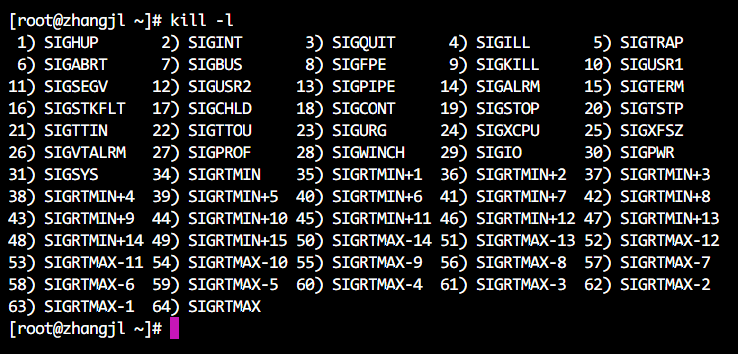
\includegraphics[width=\linewidth]{signal.png}
  \caption{Linux的信号种类}
  \label{fig:signal}
\end{figure}

使用信号,可以简单的实现kill的功能。在实现kill命令功能的时候,需要使用kill函数,具体示例如下:
\begin{code-block}{c}
#include <stdio.h>
#include <stdlib.h>
#include <signal.h>

int main(int argc, char *argv[])
{
        if(argc != 3)
        {
                printf("Usage kill signal pid\n");
                return -1;
        }
        int sig = 0, pid = 0;
        sig = atoi(argv[1]);
        pid = atoi(argv[2]);
        printf("sig is %d and pid in %d\n", sig, pid);
        kill(pid, sig);
        return 0;
}
\end{code-block}

除了使用kill进行信号的发送之外,还可以使用其他的函数进行信号的发送,比如常用的的raise,alarm等;信号的接收,通常采用pause,sleep
以及while(1)等方式;而信号的处理则通常交给signal进行。

Raise函数只会发送信号给自己,基本上等价于kill(getpid(), sig),即希望通过内核给自己发信号,常用于杀掉自身的进程,如下
\begin{code-block}{c}
#include <stdio.h>
#include <signal.h>

int main(int argc, char *argv[])
{
        printf("Raise before\n");
        raise(9);
        printf("Raise after\n");
        return 0;
}
\end{code-block}

上述代码,在编译之后运行,只有before能够输出,raise调用之后,自身进程被直接杀死,因此后续的after无法输出。

而alarm函数只会发送一个定时器信号,当程序接收到定时器信号之后,会终止对应的进程,如下:
\begin{code-block}{c}
#include <stdio.h>
#include <unistd.h>

int main(int argc, char * argv[])
{
        printf("Alarm Before\n");
        alarm(9);
        while(1); //等待9秒之后,该进程自动被终止
        printf("Alarm After\n");
        return 0;
}
\end{code-block}

因此,上述代码当中,after也是无法进行输出的。

而信号的接收,处理方式则有些不同。Pause函数会直接暂停当前的进程,如下:
\begin{code-block}{c}
#include <stdio.h>
#include <unistd.h>

int main(int argc, char * argv[])
{
        printf("Pause Before\n");
        pause();
        printf("Pause After\n");
        return 0;
}
\end{code-block}

Pasue函数一旦调用,则对应的进程会直接变为暂停状态,ps -ajx可以看到状态变为S。退出暂停状态的进程,可以直接使用Ctrl+C进行,而Ctrl+C本身
发送的就是一个终止信号。

上述的信号处理,通用的方式都是终止/暂停对应的进程,很明显并不是所有的场景都需要。因此,如何进行信号处理的自定义呢?我们需要采用signal
函数。Signal函数的定义如下:
\begin{code-block}{c}
void (*signal(int sig, void (*func)(int)))(int);
\end{code-block}

其中,func为一个函数指针,指向自定义的型号处理函数。除了自定义的信号处理函数之外,func这个函数指针还可以的取值为SIG\_IGN(忽略该信号)
和SIG\_DFL(采用系统默认方式处理信号)。简单的signal函数的使用如下:
\begin{code-block}{c}
#include <stdio.h>
#include <unistd.h>
#include <signal.h>

static int quit = 0;
void handler(int signalnum)
{
        printf("Recevied signal %d\n", signalnum);
        quit = 1;
}

int main(int argc, char * argv[])
{
        signal(SIGALRM, handler);
        alarm(9);
        while(!quit);
        printf("Using self defined function to handle signal\n");
        return 0;
}
\end{code-block}

Signal函数在用于子进程的退出处理当中,是比较常用的,比如:
\begin{code-block}{c}
#include <stdio.h>
#include <unistd.h>
#include <signal.h>
#include <stdlib.h>
#include <sys/wait.h>

void handler(int signum)
{
        int i = 0;
        while( i < 5)
        {
                printf("Receved signum %d\n", signum);
                i++;
        }
}

void clean(int signum)
{
        printf("Recevied signum %d, clean up the child process\n", signum);
        wait(NULL); // 需要使用wait函数,回收对应的进程,否则,子进程会成为僵尸进程
}

int main(int argc, char * argv[])
{
        pid_t pid;
        pid = fork();
        signal(SIGUSR1, handler);
        signal(SIGCHLD, clean);
        if (0 < pid)
        {
                int i =0;
                while(1)
                {
                        printf("This is the parent process [%d]\n", i++);
                        sleep(1);
                }
        }
        if(0 == pid)
        {
                sleep(5);
                //kill(getpid(), SIGUSR1);
                raise(SIGUSR1); // 可以直接替代上面的kill函数
                exit(0); // kill(getpid(), SIGCHLD); // 在子进程当中调用exit函数
                                                     // 相当于调用了kill函数,只不过
                                                     // 发送的信号是SIGCHLD,即杀死子进程
        }
        return 0;
}
\end{code-block}

需要注意,无名管道,命名管道以及信号,都是发生在内核空间当中,并没有发生在用户空间。
除了使用上述的方式实现进程间通信之外,在Linux当中,还可以使用IPC实现。而IPC对象包含了3种方式:
\begin{itemize}
  \item 共享内存
  \item 消息队列
  \item 信号量/灯
\end{itemize}

这些IPC对象同样是在内核空间,并没有发生在用户空间,IPC类似于Linux的文件IO操作的相关思想,可以针对文件IO与IPC做一个简单的类比,
如图\colorunderlineref{fig:IPC}所示
\begin{figure}[H]
  \centering
  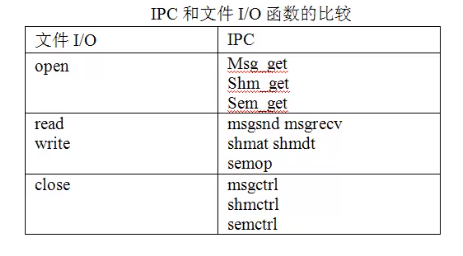
\includegraphics[width=\linewidth]{IPC.png}
  \caption{文件IO与IPC的对比}
  \label{fig:IPC}
\end{figure}

\subsection{共享内存}
共享内存通常需要使用shmget函数进行创建,而这个函数包含3个参数:
\begin{itemize}
  \item key:IPC\_PRIVATE或者是ftok函数的返回值
  \item size:共享内存的大小,bit
  \item shmflg:共享内存的权限,同open函数
\end{itemize}
共享内存的具体使用示例如下:
\begin{code-block}{c}
#include <stdio.h>
#include <sys/shm.h>

int main(int argc, char * argv[])
{
        int shmid = 0;
        if (0 > (shmid = shmget(IPC_PRIVATE, 128, 0777)))
        {
                printf("Create shared memory failed\n");
                return -1;
        }
        return 0;
}
\end{code-block}

共享内存创建完毕之后,可以直接使用Linux提供的命令进行查看和删除。
\begin{code-block}{c}
# 查看IPC对象,包括共享内存, 或者直接ipcs
ipcs -m -q -s
# 删除IPC对象
ipcrm -m <id>
\end{code-block}
在上述代码当中,创建共享内存使用的是IPC\_PRIVATE这个宏,因此,创建出来的共享内存的
key永远为0。可以改为使用ftok函数,给不同的共享内存分配不同的标识符(key),如下:
\begin{code-block}{c}
#include <stdio.h>
#include <sys/shm.h>
#include <sys/ipc.h>

int main(int argc, char * argv[])
{
        int shmid = 0;
        int key = ftok("sharedmem.c", 's');
        if (0 > key)
        {
                printf("Failed to create shamred memory key\n");
                return -1;
        }
        if (0 > (shmid = shmget(key, 128, IPC_CREAT | 0777)))
        {
                printf("Create shared memory failed\n");
                return -1;
        }
        printf("Shared memory object id is %d\n", shmid);
        return 0;
}
\end{code-block}

IPC\_PRIVATE与ftok创建的共享内存,其关系类似与无名管道和命名管道,也就是说,IPC\_PRIVATE只能用于有亲缘关系的进程间通信,
而ftok的共享内存,则是任意进程间都可以进行通信。共享内存创建完成之后,整个是放在内核空间的,因此,用户空间无法访问,但是,
可以通过映射的方式,将共享内存将这些共享内存映射到用户空间,用户空间可以直接操作这些内存。共享内存的映射,需要使用函数shmat实现。
Shmat函数包含3个参数:id表示共享内存的id号,shmaddr表示映射的地址,NULL表示自动分配,shmflg表示映射内存的权限,0可读可写。
与管道不同,共享内存是可以反复读取的,并且,一直存在与内核当中,直到被删除或者系统关闭。

而共享内存的删除,包含了2部分的操作:1是断开与用户空间的内存映射,这个操作可以使用shmdt函数实现;2是回收内核空间当中的共享内存,
需要使用函数shmctl函数进行操作。Shmctl函数的参数如下:
\begin{itemize}
  \item hmid:表示共享内存的id
  \item cmd:表示针对共享内存的操作,可选的有3个,IPC\_STAT,获取对象属性,IPC\_SET,设置对象属性,以及IPC\_RMID删除共享内存对象
  \item buf:当cmd为IPC\_SET或IPC\_STAT时,需要使用该参数表示对象属性
\end{itemize}

共享内存的整体使用,如下示例:
\begin{code-block}{c}
#include <stdio.h>
#include <sys/shm.h>
#include <sys/ipc.h>

int main(int argc, char * argv[])
{
        int shmid = 0;
        int key = ftok("sharedmem.c", 's');
        if (0 > key)
        {
                printf("Failed to create shamred memory key\n");
                return -1;
        }
        if (0 > (shmid = shmget(key, 128, IPC_CREAT | 0777)))
        {
                printf("Create shared memory failed\n");
                return -1;
        }
        printf("Shared memory object id is %d\n", shmid);
        char * buffer = NULL;
        if (NULL == (buffer = (char *)shmat(shmid, NULL, 0)))
        {
                printf("Cannot mapping shared memory to user namespace\n");
                return -1;
        }

        fgets(buffer, 128, stdin);
        printf("Shared memory data :%s\n", buffer);

        shmdt(buffer); // 删除用户空间的共享内存映射
        buffer = NULL;

        shmctl(shmid, IPC_RMID, NULL); // 删除内核空间的共享内存

        return 0;
}
\end{code-block}

共享内存也常常用于进程间通信,比如父子进程之间的通信,如下所示:
\begin{code-block}{c}
#include <stdio.h>
#include <sys/shm.h>
#include <sys/ipc.h>
#include <unistd.h>
#include <signal.h>

void parent_handler(int signum)
{
}

void child_handler(int signum)
{
}

int main(int argc, char * argv[])
{
        int shmid = 0;
        pid_t pid = 0;
        if (0 > (shmid = shmget(IPC_PRIVATE, 128, 0777)))
        {
                printf("Create shared memory failed\n");
                return -1;
        }
        printf("Shared memory object id is %d\n", shmid);

        pid = fork();
        char * buffer = NULL;
        if (0 < pid)
        {
                signal(SIGUSR2, parent_handler);
                printf("In parent process\n");
                if (NULL == (buffer = (char *)shmat(shmid, NULL, 0)))
                {
                        printf("Cannot mapping shared memory to user namespace in parent process\n");
                        return -1;
                }
                while(1)
                {
                        fgets(buffer, 128, stdin);
                        kill(pid, SIGUSR1); // 发送信号给子进程,唤醒子进程
                        pause(); // 暂停
                }
        }

        if (0 == pid)
        {
                signal(SIGUSR1, child_handler);
                if (NULL == (buffer = (char *)shmat(shmid, NULL, SHM_RDONLY)))
                {
                        printf("Cannot mapping shared memory to user namespace in child process\n");
                        return -1;
                }
                while(1)
                {
                        pause();
                        printf("The shared memory data is %s\n", buffer);
                        kill(getppid(), SIGUSR2); //发送信号给主进程,唤醒主进程
                }
        }

        shmdt(buffer);
        buffer = NULL;

        shmctl(shmid, IPC_RMID, NULL);

        return 0;
}
\end{code-block}

共享内存也可以使用实现没有亲缘关系的进程间的通信,示例如下:
\begin{code-block}{c}
// 服务端的代码
#include <stdio.h>
#include <sys/shm.h>
#include <sys/ipc.h>
#include <signal.h>
#include <stdlib.h>
#include <unistd.h>

typedef struct _buffer{
        int pid;
        char buf[128];
}buffer_t;

void hanlder(int signum){}

int main(int argc, char * argv[])
{
        signal(SIGUSR2, hanlder);
        pid_t pid = 0;
        int shmid = 0;
        buffer_t *buffer = NULL;

        int key = ftok("server.c", 's');
        if (0 > key)
        {
                printf("Failed to create shamred memory key\n");
                return -1;
        }
        if (0 > (shmid = shmget(key, sizeof(buffer_t), IPC_CREAT | 0777)))
        {
                printf("Create shared memory failed\n");
                return -1;
        }
        if (NULL == (buffer = (buffer_t *)shmat(shmid, NULL, 0)))
        {
                printf("Mapping shared memory failed \n");
                return -1;
        }

        buffer->pid = getpid(); // 通过共享内存,向客户端发送自己的pid
        pause(); // 等待客户端的输入,等待信号SIGUSR2唤醒
        pid = buffer->pid; // 获得客户端的pid

        while(1)
        {
                printf("Server process start write share memory\n");
                fgets(buffer->buf, 128, stdin);
                kill(pid, SIGUSR1); // 使用信号SIGUSR1唤醒客户端
                pause();
        }

        shmdt(buffer);
        buffer = NULL;
        shmctl(shmid, IPC_RMID, NULL);

        return 0;
}

// 客户端代码
#include <stdio.h>
#include <sys/shm.h>
#include <sys/ipc.h>
#include <signal.h>
#include <stdlib.h>
#include <unistd.h>

typedef struct _buffer{
        int pid;
        char buf[128];
}buffer_t;

void handler(int signum){}

int main(int argc, char * argv[])
{
        signal(SIGUSR1, handler);
        int shmid = 0;
        buffer_t *buffer = NULL;

        pid_t pid = 0;
        int key = ftok("server.c", 's');
        if (0 > key)
        {
                printf("Failed to create shamred memory key\n");
                return -1;
        }
        if (0 > (shmid = shmget(key, sizeof(buffer_t), IPC_CREAT | 0777)))
        {
                printf("Create shared memory failed\n");
                return -1;
        }
        if (NULL == (buffer = (buffer_t *)shmat(shmid, NULL, 0)))
        {
                printf("Mapping shared memory failed \n");
                return -1;
        }

        pid = buffer->pid; // 通过共享内存获取服务端的pid
        buffer->pid = getpid(); // 输入客户端本身的pid
        kill(pid, SIGUSR2); // 使用信号SIGUSR2唤醒服务端

        while(1)
        {
                pause();
                printf("Client process recevied data from shared memory: %s\n",
                        buffer->buf);
                kill(pid, SIGUSR2);
        }

        shmdt(buffer);
        buffer = NULL;
        shmctl(shmid, IPC_RMID, NULL);

        return 0;
}
\end{code-block}

\subsection{消息队列}
消息队列和管道不一样,它是一种双端循环链表数据结构实现的对象;不过消息队列与共享内存同属于IPC对象,因此,大部分的宏定义对于消息队列都是通用的。
消息队列的创建和删除示例如下(注意,消息队列无法在WSL1下运行):
\begin{code-block}{c}
#include <stdio.h>
#include <sys/msg.h>

int main(int argc, char * argv[])
{
        int msgid = 0;
        if (0 > (msgid = msgget(IPC_PRIVATE, 0777)))
        {
                printf("Faild to create msg queue\n");
                return -1;
        }
        printf("Msg queue id is %d\n", msgid);
        msgctl(msgid, IPC_RMID, NULL);
        return 0;
}
\end{code-block}

消息队列创建成功之后,就可以向其中进行消息的发送和收取。其中消息的发送需要使用函数msgsnd,该函数包含了4个参数:
\begin{itemize}
  \item msgid:消息队列的id
  \item msgp:指向消息的指针
  \item size:发送的消息正文的字节数
  \item flag:IPC\_NOWAIT,消息没有发送完成,函数也立即返回;0表示必须等待消息发送完毕之后,才返回
\end{itemize}
特别需要注意的是,消息通常使用结构体进行表述,其中至少需要包含2个要素:1是消息的类型;2是消息的正文。常见的消息结构体如下:
\begin{code-block}{c}
struct msgbuf{
        long mtype; // 消息类型
        char mtext[N]; // 消息正文,size的大小就表示该元素的长度
};
\end{code-block}
注意,消息结构体最好只包含上述的元素,如果需要使用额外的字段,或者包含其他的结构体,则必须将其他字段放在
上述结构体原本必须存在的字段的后面,否则可能导致消息无法被读取。合理的自定义消息结构体如下:
\begin{code-block}{c}
struct msgbuf{
        long msgtype;
        char msgtext[N];
        int msgid;
        struct {
            char * child_name;
            uint8_t child_age;
        };
};
\end{code-block}

消息发送到消息队列之后,就可以从消息队列当中进行读取了。读取消息队列当中的内容,需要使用msgrcv函数,该函数包含了5个参数:
\begin{itemize}
  \item msgid:消息队列的id
  \item msgp:指向消息的指针,同消息发送的参数
  \item size:接收的消息正文字节数
  \item msgtype:0表示接受消息队列当中的第一个消息;>0表示接收消息队列当中第一个类型为msgtype的消息;<0表示接收消息队列中类型值不大于msgtype绝对值,但是类型值最小的消息
  \item flag:0表示没有消息则一直阻塞;IPC\_NOWAIT表示如果没有消息,则立即返回ENOMSG
\end{itemize}

特别注意的是,如果使用的是自定义的消息结构体,并且需要读取消息结构体当中的其他字段内容,则发送和接收时,size的大小需要进行变更,
不再是msgtext的大小,而是消息结构体的整体大小。

消息队列简单的示例如下:
\begin{code-block}{c}
#include <stdio.h>
#include <sys/msg.h>
#include <string.h>

typedef struct _msgbuffer{
        long msgtype;
        char mtext[128]; // 第一个和第二个字段必须为long和char,否则,调用msgrcv会无法收到任何消息
        int msgid;
        struct {
            char * child_name;
            unsigned char child_age;
        };
}msgbuffer_t;

int main(int argc, char * argv[])
{
        int msgid = 0;
        if (0 > (msgid = msgget(IPC_PRIVATE, 0777)))
        {
                printf("Faild to create msg queue\n");
                return -1;
        }

        printf("Msg queue id is %d\n", msgid);

        msgbuffer_t buffer, recv;
        buffer.msgtype = 100;
        memset(buffer.mtext, 0, 128);
        strcpy(buffer.mtext, "hello");
        buffer.child_name = "lucifer";
        buffer.child_age = 18;
        buffer.msgid = 18;
        msgsnd(msgid, &buffer, sizeof(buffer), 0);

        memset(recv.mtext, 0, 128);
        int readret = msgrcv(msgid, &recv,
                sizeof(recv), 100, 0);
        printf("Recv msg :%s\n", recv.mtext);
        printf("Read size %d\n", readret);
        printf("Msg.msgid :%d, msg.child_name: %s, msg.child_age: %d\n",
            recv.msgid, recv.child_name, recv.child_age);

        msgctl(msgid, IPC_RMID, NULL);
        return 0;
}
\end{code-block}

消息队列可以实现无亲缘关系的进程间的通信,包括半双工和双工通信。简单的半双工通信方式如下:
\begin{code-block}{c}
// server端的代码
#include <stdio.h>
#include <sys/msg.h>
#include <string.h>
#include <unistd.h>

typedef struct _msgbuffer{
        long msgtype;
        char mtext[128];
        int msgid;
        struct {
            char * child_name;
            unsigned char child_age;
        };
}msgbuffer_t;

int main(int argc, char * argv[])
{
        int msgid = 0;
        int ipckey= 0;
        if (0 > (ipckey = ftok("/var/run", 'r')))
        {
                printf("Failed to create ipc key\n");
                return -1;
        }
        if (0 > (msgid = msgget(ipckey, IPC_CREAT|0777)))
        {
                printf("Faild to create msg queue\n");
                return -1;
        }

        printf("Msg queue id is %d\n", msgid);

        msgbuffer_t buffer;
        buffer.msgtype = 1;
        while(1)
        {
                memset(buffer.mtext, 0, 128);
                strcpy(buffer.mtext, "This is a message");
                buffer.child_name = "lucifer";
                buffer.child_age = 18;
                buffer.msgid = 0;
                msgsnd(msgid, &buffer, sizeof(buffer), 0);
                sleep(2);
        }

        msgctl(msgid, IPC_RMID, NULL);
        return 0;
}

// client端的代码
#include <stdio.h>
#include <sys/msg.h>
#include <string.h>
#include <unistd.h>

typedef struct _msgbuffer{
        long msgtype;
        char mtext[128];
        int msgid;
        struct {
            char * child_name;
            unsigned char child_age;
        };
}msgbuffer_t;

int main(int argc, char * argv[])
{
        int msgid = 0;
        int ipckey= 0;
        if (0 > (ipckey = ftok("/var/run", 'r')))
        {
                printf("Failed to create ipc key\n");
                return -1;
        }
        if (0 > (msgid = msgget(ipckey, IPC_CREAT|0777)))
        {
                printf("Faild to create msg queue\n");
                return -1;
        }

        printf("Msg queue id is %d\n", msgid);

        msgbuffer_t buffer;
        int readret = 0;
        while(1)
        {
                readret = msgrcv(msgid, &buffer,
                        sizeof(msgbuffer_t), 1, 0);
                printf("Recv msg :%s\n", buffer.mtext);
                printf("Read size %d\n", readret);
                printf("msg.child_name: %s, msg.child_age: %d, msg.msgid: %d\n",
                        buffer.child_name, buffer.child_age, buffer.msgid);
        }

        msgctl(msgid, IPC_RMID, NULL);
        return 0;
}
\end{code-block}

而消息队列的全双工通信模式的代码基本如下:
\begin{code-block}{c}
// sever端的代码
#include <stdio.h>
#include <sys/msg.h>
#include <string.h>
#include <unistd.h>

typedef struct _msgbuffer{
        long msgtype;
        char mtext[128];
        int msgid;
        struct {
            char * child_name;
            unsigned char child_age;
        };
}msgbuffer_t;

int main(int argc, char * argv[])
{
        int msgid = 0;
        int ipckey= 0;
        if (0 > (ipckey = ftok("/var/run", 'r')))
        {
                printf("Failed to create ipc key\n");
                return -1;
        }
        if (0 > (msgid = msgget(ipckey, IPC_CREAT|0777)))
        {
                printf("Faild to create msg queue\n");
                return -1;
        }

        printf("Msg queue id is %d\n", msgid);

        pid_t pid = 0;
        if (0 < (pid = fork()))
        {
                msgbuffer_t buffer;
                buffer.msgtype = 1;
                while(1)
                {
                        memset(buffer.mtext, 0, 128);
                        strcpy(buffer.mtext,
                                "Hello client, this is server");
                        buffer.child_name = "lucifer";
                        buffer.child_age = 18;
                        buffer.msgid = 0;
                        msgsnd(msgid, &buffer, sizeof(buffer), 0);
                        sleep(5);
                }
        }
        if (0==pid)
        {
                msgbuffer_t buffer;
                int readret = 0;
                while(1)
                {
                        memset(buffer.mtext, 0, 128);
                        readret = msgrcv(msgid,
                                &buffer, sizeof(msgbuffer_t), 2, 0);
                        printf("Recv msg :%s\n", buffer.mtext);
                        printf("Read size %d\n", readret);
                        printf("Recv data child_age: %d\n",
                                buffer.child_age);
                }
        }


        msgctl(msgid, IPC_RMID, NULL);
        return 0;
}


// 客户端代码
#include <stdio.h>
#include <sys/msg.h>
#include <string.h>
#include <unistd.h>

typedef struct _msgbuffer{
        long msgtype;
        char mtext[128];
        int msgid;
        struct {
            char * child_name;
            unsigned char child_age;
        };
}msgbuffer_t;

int main(int argc, char * argv[])
{
        int msgid = 0;
        int ipckey= 0;
        if (0 > (ipckey = ftok("/var/run", 'r')))
        {
                printf("Failed to create ipc key\n");
                return -1;
        }
        if (0 > (msgid = msgget(ipckey, IPC_CREAT|0777)))
        {
                printf("Faild to create msg queue\n");
                return -1;
        }

        printf("Msg queue id is %d\n", msgid);

        pid_t pid = 0;
        if(0 < (pid=fork()))
        {
                msgbuffer_t buffer;
                int readret = 0;
                while(1)
                {
                        readret = msgrcv(msgid, &buffer,
                                sizeof(msgbuffer_t), 1, 0);
                        printf("Recv msg :%s\n", buffer.mtext);
                        printf("Read size %d\n", readret);
                }

        }
        if (0 == pid)
        {
                msgbuffer_t buffer;
                buffer.msgtype = 2;
                while(1)
                {
                        memset(buffer.mtext, 0, 128);
                        strcpy(buffer.mtext,
                                "Hello server, this is client");
                        buffer.child_name = "lucifer";
                        buffer.child_age = 18;
                        buffer.msgid = 0;
                        msgsnd(msgid, &buffer, sizeof(buffer), 0);
                        sleep(5);
                }
        }

        msgctl(msgid, IPC_RMID, NULL);
        return 0;
}
\end{code-block}

\subsection{信号量/灯}
信号灯是信号量的集合,可以含有多个信号量。信号灯的创建需要使用函数semget,该函数总共有3个参数,其含义如下:
\begin{itemize}
  \item key\_t:与型号等级关联的key值,可以使用IPC\_PRIVATE和ftok,与其他的ipc对象相同
  \item nsems:信号灯集所包含的信号灯数量
  \item semflg:信号灯集的访问权限
\end{itemize}
而信号灯的删除,则需要使用semctl函数,该函数与其他的ipc对象的操作类似:
\begin{itemize}
  \item semid:信号灯集的id
  \item semnum:要改变的信号灯的编号
  \item cmd:GETVAL,获取信号灯的值;SETVAL,设置信号灯的值;IPC\_RMID,删除信号灯集合
  \item semun arg:修改或获取信号灯的属性时需要,本身为可选参数
\end{itemize}
信号灯的简单创建和删除,如下:
\begin{code-block}{c}
#include <stdio.h>
#include <sys/sem.h>

int main(int argc, char * argv[])
{
        int semid = 0;
        if (0 > (semid = semget(IPC_PRIVATE, 3, 0777)))
        {
                printf("Faild to create sem \n");
                return -1;
        }
        printf("sem id is %d\n", semid);
        semctl(semid, 0, IPC_RMID); // 等效于semctl(semid, 0, IPC_RMID,NULL);
        return 0;
}
\end{code-block}

信号灯集可以在进程间,也可以在线程间进行通信。如下的,在线程中通信使用信号灯:
\begin{code-block}{c}
#include <stdio.h>
#include <pthread.h>
#include <unistd.h>
#include <sys/sem.h>
#include <sys/ipc.h>
#include <stdlib.h>

int semid = 0;

typedef union _semun {
        int val;
        struct semid_ds *buf;
        unsigned short  *array;
        struct seminfo  *__buf;
}semun_u;

struct sembuf sbuf;

void * func(void * var)
{
        int i = 0;
        sbuf.sem_op = -1;
        semop(semid, &sbuf, 1);
        while(i< 10)
        {
                usleep(100);
                printf("This is func i=%d\n", i++);
        }
}

int main(int argc, char * argv[])
{
        int i = 0;
        char buf[] = "hello world";
        pthread_t tid = 0;
        int ret = 0;
        if (0 > (semid = semget(IPC_PRIVATE, 3, 0777)))
        {
                printf("Failed to create sem\n");
                return -1;
        }
        printf("%d\n", sizeof(buf));
        semun_u se;
        se.val = 0;
        semctl(semid, 0, SETVAL, se);
        sbuf.sem_flg = 0;
        sbuf.sem_num = 0;

        if(0 > (ret = pthread_create(&tid, NULL, func, buf)))
        {
                printf("Failed to create thread \n");
                return -1;
        }

        while(i < 10)
        {
                usleep(100);
                printf("This is man fun i=%d\n",i++);
        }
        sbuf.sem_op = 1;
        semop(semid, &sbuf, 1);
        sleep(5);
        return 0;
}

// 信号量的版本
#include <stdio.h>
#include <pthread.h>
#include <unistd.h>
#include <semaphore.h>

sem_t sem;

void * func(void * var)
{
        int i = 0;
        sem_wait(&sem);
        while(i< 10)
        {
                usleep(100);
                printf("This is func i=%d\n", i++);
        }
}

int main(int argc, char * argv[])
{
        int i = 0;
        char buf[] = "hello world";
        pthread_t tid = 0;
        int ret = 0;
        sem_init(&sem, 0, 0);
        if(0 > (ret = pthread_create(&tid, NULL, func, buf)))
        {
                printf("Failed to create thread \n");
                return -1;
        }

        while(i < 10)
        {
                usleep(100);
                printf("This is man fun i=%d\n",i++);
        }
        sem_post(&sem);
        sleep(5);
        return 0;
}
\end{code-block}

由于使用了pthread,因此,编译的时候,需要加上参数:
\begin{code-block}{bash}
gcc -pthread -o sem sem.c
\end{code-block}

信号量也可以用于进程间的通信,具体的可见如下示例:
\begin{code-block}{c}
// 服务器端
#include <stdio.h>
#include <sys/sem.h>

typedef union _semun {
        int val;
        struct semid_ds *buf;
        unsigned short  *array;
        struct seminfo  *__buf;
}semun_u;

int main(int argc, char * argv[])
{
        key_t key = 0;
        if (0 > (key = ftok("/var/run", 'v')))
        {
                printf("Failed to creat key\n");
                return -1;
        }
        int semid = 0;
        if (0 > (semid = semget(key, 3, IPC_CREAT|0777)))
        {
                printf("Failed to create sem\n");
                return -1;
        }
        //semun_u se;
        //se.val = 0;
        //semctl(semid, 0, SETVAL, se);

        struct sembuf sbuf;
        sbuf.sem_flg = 0;
        sbuf.sem_num = 0;

        int i = 0;
        while(i < 10)
        {
                usleep(100);
                printf("This is man fun i=%d\n",i++);
        }
        sbuf.sem_op = 1;
        semop(semid, &sbuf, 1);
        return 0;
}

// 客户端
#include <stdio.h>
#include <sys/sem.h>

typedef union _semun {
        int val;
        struct semid_ds *buf;
        unsigned short  *array;
        struct seminfo  *__buf;
}semun_u;

struct sembuf sbuf;

int main(int argc, char * argv[])
{
        key_t key = 0;
        if (0 > (key = ftok("/var/run", 'v')))
        {
                printf("Failed to creat key\n");
                return -1;
        }
        int semid = 0;
        if (0 > (semid = semget(key, 3, IPC_CREAT|0777)))
        {
                printf("Failed to create sem\n");
                return -1;
        }
        semun_u se;
        se.val = 0;
        semctl(semid, 0, SETVAL, se);
        sbuf.sem_flg = 0;
        sbuf.sem_num = 0;
        sbuf.sem_op = -1;
        semop(semid, &sbuf, 1);

        int i = 0;
        while(i < 10)
        {
                usleep(100);
                printf("This is man fun i=%d\n",i++);
        }
        return 0;
}
\end{code-block}

\section{多线程}
进程是一个正在执行的程序,是资源分配的最小单位。进程需要按照一定的循序逐次执行。线程称之为轻量级的进程,是程序执行的最小单位,系统
独立调度和分配cpu的基本单位,是进程中的一个实体。一个进程可以有多个线程,所有线程共享进程的所有资源。进程是资源的拥有者,但是,创建,
删除以及切换需要消耗较大的时间和空间开销,并且子进程需要复制父进程的所有资源;而对称多处理机(SMP)可以满足多个运行单位。
获取线程id的方式如下:
\begin{code-block}{c}
#include <stdio.h>
#include <unistd.h>
#include <pthread.h>

int main(int argc, char * argv[])
{
        pid_t pid = 0;
        pthread_t tid = 0;
        pid = getpid();
        tid = pthread_self();
        printf("The pid is %u and tid is %x\n", pid, tid);
        return 0;
}
\end{code-block}

需要注意的是,pthread\_id在Linux当中是整形的别名,但是Unix当中是结构体,2者不一样。线程的创建需要使用函数pthread\_create,该函数有4个参数:
\begin{itemize}
  \item thread:如果创建成功,返回的新线程的id
  \item attr:线程属性,包括调度策略,继承性和分离性
  \item start\_routine:回调函数,即新线程需要执行的功能
  \item arg:回调函数的参数
\end{itemize}
如果线程传递成功,则返回0, 反之返回错误码。简单的示例如下:
\begin{code-block}{c}
#include <stdio.h>
#include <pthread.h>
#include <unistd.h>

void print_id(char * s)
{
        pid_t pid;
        pthread_t tid;
        pid = getpid();
        tid = pthread_self();
        printf("%s Pid is %u, and tid is %x\n", s, pid, tid);
}

void * fun(void * arg)
{
        print_id(arg);
        return NULL;
}

int main(int argc, char * argv[])
{
        pthread_t npid;
        int err = 0;
        if (err=pthread_create(&npid, NULL, fun, "newthread"))
        {
                printf("Faild to creat thread\n");
                return -1;
        }
        print_id("main thread");
        int ret = 0;
        pthread_exit(&ret);
        return 0;
}
\end{code-block}

程序运行时,首先运行的是main函数,即主线程或称之为初始线程。在初始线程当中,可以做任何普通线程可以做的事情。但是,主线程在main函数返回或者退出的时候,
会导致进程结束,因此,通常的,需要在主线程当中调用pthread\_exit函数,等待所有线程结束之后才终止。绝大多数情况下,主线程在默认堆栈上
运行,但是普通线程的堆栈,是受限制的,一旦溢出,就会出现错误。

主线程是随着进程的创建而创建的,新的线程可能在pthread\_create返回之前就已经运行,甚至运行完毕了。多线程也可以进行结构体的传递,如下:
\begin{code-block}{c}
#include <stdio.h>
#include <pthread.h>
#include <unistd.h>

typedef struct _student {
        unsigned char age;
        char name[32];
}student_t;

// 定义函数指针别名,如果不如此定义,则线程的函数,则必须写作
// void * func (void *)的形式,需要在线程函数内部做类型的强制类型转换
typedef void *(*start_routine)(void *);

void * printstu(student_t * stu_t)
{
        printf("The student info is name :%s, and age: %d\n",
                stu_t->name, stu_t->age);
        return NULL;
}

int main(int argc, char * argv[])
{
        pthread_t npid;
        int err = 0;
        student_t stu = {18, "zhangjl"};
        if (err=pthread_create(
                &npid, NULL, (start_routine)printstu, &stu))
        {
                printf("Faild to creat thread\n");
                return -1;
        }
        int ret = 0;
        pthread_exit(&ret);
        return 0;
}
\end{code-block}

与进程一样,线程也有自己的状态:
\begin{itemize}
  \item 就绪:线程能够运行,但在等待可用的处理器
  \item 运行:线程正在运行
  \item 阻塞:线程在等待其他条件就绪
  \item 终止:线程声明周期结束
\end{itemize}
线程的状态转换如图\colorunderlineref{fig:status_of_thread}所示
\begin{figure}[H]
  \centering
  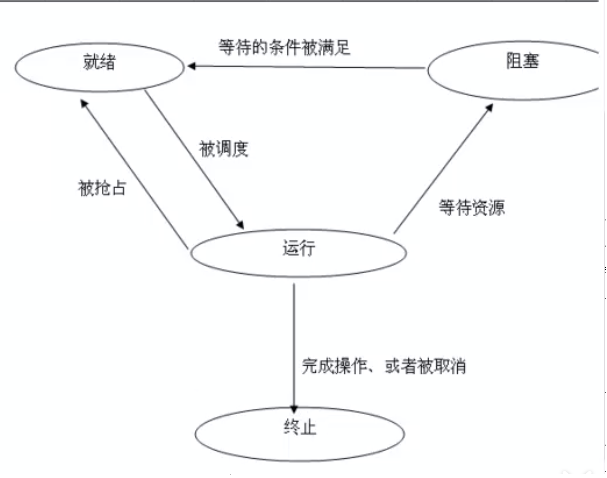
\includegraphics[width=\linewidth]{status_of_thread.png}
  \caption{线程的状态转换}
  \label{fig:status_of_thread}
\end{figure}

线程的分离属性:分离一个正在运行的线程并不影响他,仅仅是通知当前系统,如果该线程结束,其所属的资源可以回收;一个没有被分离的线程在终止时
会保留它的虚拟内存,包括对应的堆栈和其他系统资源,这种线程通称为僵尸线程。需要注意的是,线程创建时,默认是非分离的。

如果线程具有分离属性,则线程终止是会被立刻回收,回收操作将释放所有在线程终止是为释放的系统资源和进程资源,包括保存线程返回值的内存空间。
终止被分离的线程会释放所有的系统资源,并且必须释放由该线程所占有的程序资源。

线程的退出最好不要使用exit函数,该函数会导致整个进程的终止。正常的线程终止操作通常如下:
\begin{itemize}
  \item 从启动线程中返回,返回值是线程的退出码
  \item 可以被同一进程的其他线程取消
  \item 调用pthread\_exit函数退出
\end{itemize}

阻塞线程通常使用pthread\_join函数,调用该函数,对应的线程会一直阻塞,直到指定的线程调用pthread\_exit,或者从启动的线程返回,或者被取消。
一点调用pthread\_join函数,会使指定的线程处于分离状态。如果调用函数pthread\_detach,也会分离线程。

